\documentclass[aspectratio=169, 11pt]{beamer}

%% ── Theme ──────────────────────────────────────────────────────
\usetheme[progressbar=frametitle]{metropolis}

%% ── Packages ───────────────────────────────────────────────────
\usepackage[T1]{fontenc}
\usepackage[utf8]{inputenc}
\usepackage{lmodern}
\usepackage[absolute,overlay]{textpos}
\usepackage{appendixnumberbeamer}
\usepackage{xcolor}
\usepackage{booktabs}
\usepackage{tikz}
\usepackage{hyperref}
\usepackage{xspace}
\usepackage{amsmath,amssymb}
\usetikzlibrary{arrows.meta,positioning,fit,backgrounds,calc}

%% ── Notes ──
\usepackage{pgfpages}
\setbeameroption{show notes on second screen=right}  % side-by-side speaker notes
% Smaller speaker-notes typography (request: notes too large on screen)
\setbeamerfont{note page}{family*=cmss,size=\scriptsize}
\setbeamerfont{note title}{family*=cmss,size=\footnotesize,series=\bfseries}

%% ── ORNL colors ────────────────────────────────────────────────
\definecolor{ornlgreen}{RGB}{0,121,52}
\definecolor{ornlblack}{RGB}{0,0,0}
\definecolor{ornlgrey}{RGB}{88,88,88}
\definecolor{backgroundgreen}{RGB}{68,126,89}
\definecolor{backgroundgrey}{RGB}{191,191,191}
\definecolor{cerulean}{RGB}{0,122,166}

\setbeamercolor{progress bar}{fg=ornlgreen, bg=ornlgreen!30}
\setbeamercolor{normal text}{fg=ornlblack, bg=white}
\setbeamercolor{frametitle}{fg=ornlblack, bg=white}
\setbeamercolor{structure}{fg=ornlgreen}
\setbeamercolor{itemize item}{fg=ornlgreen}
\setbeamercolor{block title}{fg=white, bg=ornlgreen}
\setbeamercolor{block body}{fg=ornlblack, bg=ornlgreen!8}

\usebackgroundtemplate{%
  
\includegraphics[width=\paperwidth]{style/assets/slide_frame.png}}

\newcommand{\maketitlepage}{%
  {\usebackgroundtemplate{%
     
\includegraphics[angle=0,width=\paperwidth]{style/assets/title_frame.png}}%
   \begin{frame}\titlepage\end{frame}}}
\defbeamertemplate*{title page}{customized}[1][]{%
  \setbeamertemplate{footline}{}
  \textcolor{white}{\Huge \inserttitle}\\[4pt]
  \textcolor{white}{\large \insertsubtitle}\\[14pt]
  \textcolor{white}{\Large \insertauthor}\\[4pt]
  \textcolor{white}{\insertdate}}

\hypersetup{colorlinks=true,linkcolor=blue,urlcolor=cerulean,citecolor=blue}

%% ── Compact footnote command for paper refs ────────────────────
\newcommand{\refnote}[1]{%
  \begin{textblock*}{0.95\paperwidth}(0.025\paperwidth,0.93\paperheight)
    \scriptsize\color{ornlgrey} #1
  \end{textblock*}}

%% ── Metadata ───────────────────────────────────────────────────
\title{\small AI-Agent Driven Survey and Validated Literature Review for Discovering Solid Breeder Materials}
\subtitle{End-to-End Traceability  for Automated Literature Generation}
\author{Jose Tupayachi, Gabe Parker, Xueping Li and Xiao-Ying Yu\textsuperscript{*}}


\institute{
Materials Science and Technology Division\\
\small Research supported by DOE FES
}

\date{
\tiny
ANS TOFE 2026\\
Denver, Colorado\\[4pt]
\scriptsize Research supported by DOE FES
}
\begin{document}

%% ═══════════════════════════════════════════════════════════════
%% 1 — TITLE
%% ═══════════════════════════════════════════════════════════════
\maketitlepage

\note{Good afternoon. I'm Jose Tupayachi, from ORNL. Today I'm presenting our end-to-end framework for AI-agent driven literature generation .}


\begin{frame}{AI-Agent Driven Literature Reviews with Full Claim Traceability}
\centering
\begin{columns}[c]
    \begin{column}{0.58\textwidth}
        \centering
        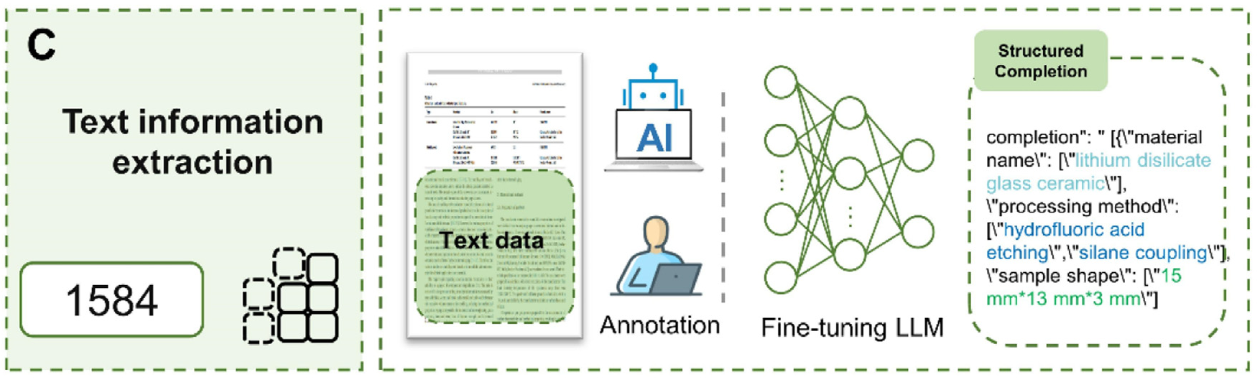
\includegraphics[width=0.95\linewidth]{newfigures/workflow.png}

        {\scriptsize\color{ornlgrey}End-to-End Generation}
    \end{column}

    \hfill

    \begin{column}{0.38\textwidth}
        \centering
        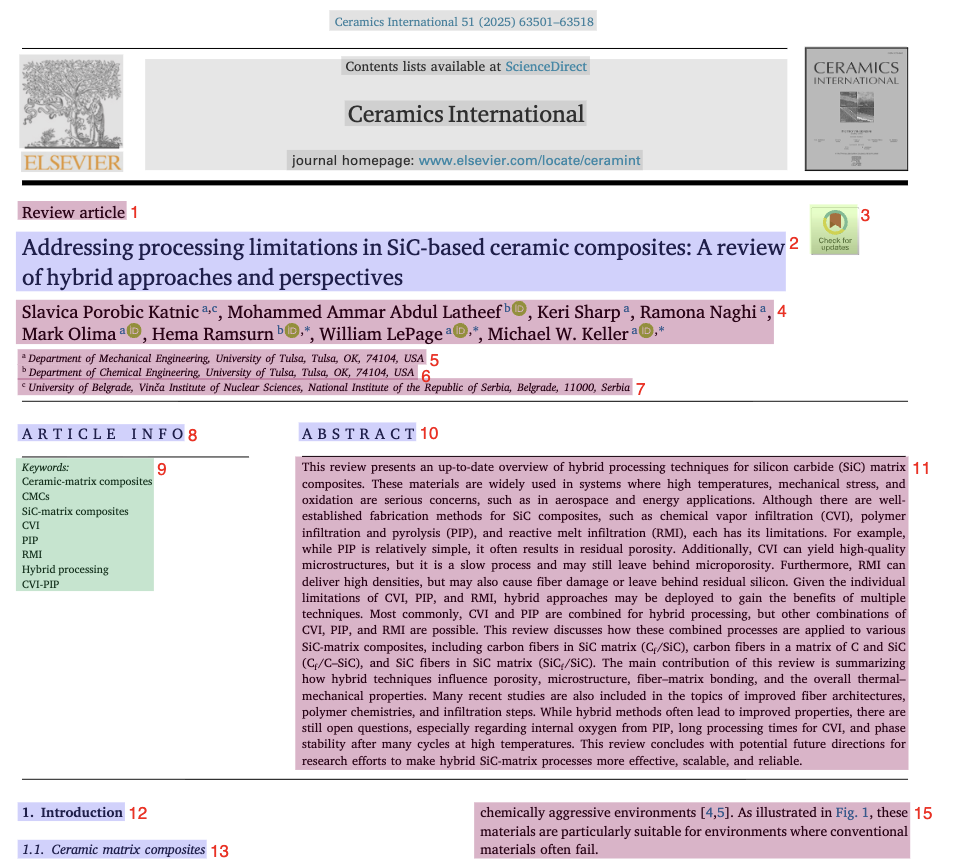
\includegraphics[width=0.95\linewidth]{newfigures/ocr.png}

        {\scriptsize\color{ornlgrey}OCR with bounding-box capture}
    \end{column}
\end{columns}
\vspace{4pt}
\begin{minipage}{0.92\linewidth}
\begin{itemize}\setlength\itemsep{1pt}
  \footnotesize
  \item \textbf{Manual reviews}: Screening hundreds of papers can take weeks to months.
  \item \textbf{Commercial platforms}: Subscription fees, token limits, and usage caps restrict scalability.
  \item \textbf{LLM-generated reviews}: Often lack transparent source attribution and traceability.
\end{itemize}
% \vspace{4pt}
\end{minipage}\\[4pt]
\textcolor{ornlgreen}{\normalsize\textbf{Our contribution: a LLM pipeline with per-claim traceability.}}
\end{frame}
\note{

Explain
% Here is the problem. A manual literature review of even a moderately sized area takes weeks of expert time. Paid tools hit token limits and pricing caps scalability. On the other hand, while generated text corpora may be coherent, there is generally no mechanism to verify the origin of each specific claim.\\


% % a generic large language model can produce a coherent-sounding narrative, but it is often difficult to verify where specific claims originated.

% Our contribution is a  pipeline where every claim in the generated manuscript links back to an exact paper, hypothesis, and research direction}
}


%% ═══════════════════════════════════════════════════════════════
%% 2b — WHY THIS STUDY MATTERS (TikZ-driven, minimal text)
%% ═══════════════════════════════════════════════════════════════
% \begin{frame}{Manual Reviews are Slow, Costly, and May Introduce Bias}
% \centering\vspace{-4pt}
% \begin{columns}[T]
%   %% ── Left: reaction (top) above solid vs liquid (bottom) ────────
%   \begin{column}{0.56\textwidth}\centering
%     \scalebox{0.82}{%
%     \begin{tikzpicture}[font=\scriptsize,
%       rx/.style={draw=ornlgreen,fill=ornlgreen!10,rounded corners=2pt,
%                  inner sep=4pt,align=center,text=ornlblack,
%                  text width=7.6cm},
%       sol/.style={draw=ornlgreen,fill=white,rounded corners=2pt,
%                   inner sep=3pt,align=left,text=ornlblack,text width=3.6cm},
%       liq/.style={draw=backgroundgrey,fill=white,rounded corners=2pt,
%                   inner sep=3pt,align=left,text=ornlblack,text width=3.6cm},
%       arrG/.style={-Stealth,ornlgreen,thick},
%       arrK/.style={-Stealth,ornlgrey,thick}]
%       \node[rx](rxn){$^{6}\!\mathrm{Li}+n \to {}^{4}\!\mathrm{He}+{}^{3}\!\mathrm{H}+\,4.78\,\mathrm{MeV}$\;\;\;\textbf{\color{ornlgreen}TBR $\geq 1.05$ required}};
%       \node[sol,below left=0.55cm and -1.85cm of rxn.south](s){\textbf{\color{ornlgreen}Solid (Li$_2$TiO$_3$, Li$_4$SiO$_4$, Li$_2$ZrO$_3$)}\\$\checkmark$ chemically stable\\$\checkmark$ low pressure\\$\checkmark$ separable from coolant};
%       \node[liq,below right=0.55cm and -1.85cm of rxn.south](l){\textbf{\color{ornlgrey}Liquid (PbLi, FLiBe)}\\$\times$ MHD pressure drop\\$\times$ corrosion of structure\\$\times$ tritium permeation};
%       \draw[arrG](rxn.south)--(s.north);
%       % \draw[arrK](rxn.south)--(l.north);
%     \end{tikzpicture}}
%   \end{column}
%   \begin{column}{0.42\textwidth}\centering
%     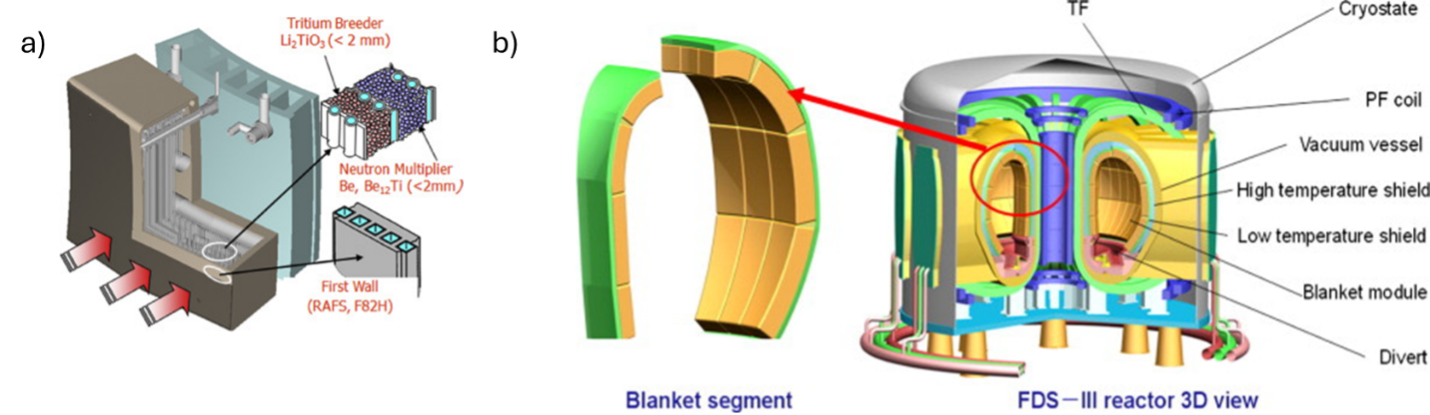
\includegraphics[width=\linewidth]{newfigures/breeder.png}\\[2pt]
%     {\scriptsize\color{ornlgrey}Blanket module with Li$_2$TiO$_3$ breeder pellets (a) and FDS-III reactor cross-section (b)}
%   \end{column}
% \end{columns}
% \vspace{10pt}

% \centering
% \scalebox{0.82}{%
% \begin{tikzpicture}[font=\tiny,
%   ev/.style={draw=ornlgreen,fill=white,rounded corners=2pt,
%              inner sep=2pt,align=center,text=ornlblack,text width=1.75cm,
%              minimum height=0.85cm},
%   arr/.style={-Stealth,ornlgrey,thick}]
%   \node[ev](e1){\textbf{1938}\\Fission discovered};
%   \node[ev,right=0.22cm of e1](e2){\textbf{1952}\\First DT fusion};
%   \node[ev,right=0.22cm of e2](e3){\textbf{1985}\\ITER concept};
%   \node[ev,right=0.22cm of e3](e4){\textbf{2007}\\ITER construction};
%   \node[ev,right=0.22cm of e4](e5){\textbf{2025}\\Blanket R\&D peak};
%   \node[ev,right=0.22cm of e5,fill=ornlgreen!15](e6){\textbf{2034}\\ITER first plasma};
%   \node[ev,right=0.22cm of e6,fill=ornlgreen!15](e7){\textbf{$\sim$2040}\\DEMO blanket};
%   \foreach \a/\b in {e1/e2,e2/e3,e3/e4,e4/e5,e5/e6,e6/e7}{\draw[arr](\a)--(\b);}
% \end{tikzpicture}}\\[2pt]

% %% ── Abbreviations footer ────────────────────────────────────────
% \vspace{12pt}
% \begin{beamercolorbox}[wd=\textwidth,sep=2pt]{block body}
%   {\tiny\color{ornlgrey}%
%    \textbf{Abbreviations:}
%    DT~=~deuterium-tritium;\;%ok
%    TBR~=~tritium breeding ratio;\;%ok
%    MHD~=~magnetohydrodynamic;\;%ok
%    PbLi~=~lead-lithium alloy;\;%ok
%    FLiBe~=~lithium fluoride--beryllium fluoride;\;%ok
%    ITER~=~International Thermonuclear Experimental Reactor;\;%ok
%    DEMO~=~demonstration power plant;\; %OK
%    % R\&D~=~research and development;\;
%    FDS-III~=~Fusion Design Study III\; %OK
%    TBR~=~tritium breeding ratio;\; %OK
%    MHD~=~magnetohydrodynamic;\; %OK
%   }
% \end{beamercolorbox}

% \end{frame}

% \note{

% % Lithium ceramics in the reactor wall absorb neutrons and produce it. Fusion reactors must breed their own tritium fuel —   Solid ceramics outperform liquid alternatives on stability, pressure, and corrosion. 

% Lithium ceramics in reactor walls absorb neutrons to produce tritium fuel. Fusion systems must breed their own fuel, and solid ceramics are preferred over liquids for their stability, corrosion resistance, and pressure tolerance.\\



% Years of breeder research span thousands of papers distributed across multiple groups and publications. Our pipeline enables researchers to directly guide this large-scale synthesis by defining two ontologies: \\

% a structural ontology and a style ontology. The structural ontology encodes the key concepts and relationships embedded in the manuscript, while the style ontology specifies how content should be written.\\}

% Years of breeder research is dispersed across many articles and research groups. Our pipeline addresses this fragmentation by allowing researchers to define a high-level structured representation—an ontology and section schema—that specifies the concepts, relationships, and organization of the manuscript. This ensures that the generated paper follows the researcher’s intended scientific framing rather than a generic narrative structure. The system then systematically reviews the literature and generates content aligned with this specification, with every claim explicitly traceable to its original source.

% Years of breeder research is fragmented across several articles and research groups. Our pipeline let researchers control the output by specifying the a high level representation know as an ontoly ontology and section structure , so the generated manuscript follows their scientific framing, not a generic one. The pipeline then sweeps the full literature and writes to that specification, with every claim traced back to its source.

%% ═══════════════════════════════════════════════════════════════
%% 3 — RELATED WORK vs OUR PROPOSAL  (combined, 5-word bullets)
%% ═══════════════════════════════════════════════════════════════
\begin{frame}{Solid Breeders are one the Bottleneck for Fusion Energy}
\vspace{4pt}

\begin{columns}[T]
  \begin{column}{0.48\textwidth}
    \centering\textbf{\color{ornlgrey}Current Approaches}\\[10pt]
    \footnotesize
    \begin{itemize}\setlength\itemsep{6pt}
      \item Analyze papers and databases individually
      \item Limited claim-level verification
      \item Static LLM prompts cannot explore research questions in depth
      \item Focus on prediction, not review generation
    \end{itemize}
  \end{column}
  \begin{column}{0.04\textwidth}\centering
    \rule{0.5pt}{4cm}
  \end{column}
  \begin{column}{0.46\textwidth}
    \centering\textbf{\color{ornlgreen}Our Approach}\\[10pt]
    \footnotesize
    \begin{itemize}\setlength\itemsep{6pt}
      % \item Integrade multimodal information (inc. ontologies()
      \item Integrate multimodal information (incl. ontologies)
      \item Verifies every sentence 
      \item Produces traceable review manuscripts automatically
      \item Graph-based approach enables deeper exploration of research questions
    \end{itemize}
  \end{column}
\end{columns}

% \begin{columns}[T]
%   \begin{column}{0.48\textwidth}
%     \centering\textbf{\color{ornlgrey}What others have done}\\[10pt]
%     \footnotesize
%     \begin{itemize}\setlength\itemsep{6pt}
%       \item Mine one source of information at a time
%       \item No line by line validation
%       \item Build static review matrices
%       \item Align Probe LLM reasoning on materials science tasks
%     \end{itemize}
%   \end{column}
%   \begin{column}{0.04\textwidth}\centering
%     \rule{0.5pt}{4cm}
%   \end{column}
%   \begin{column}{0.46\textwidth}
%     \centering\textbf{\color{ornlgreen}What we propose}\\[10pt]
%     \footnotesize
%     \begin{itemize}\setlength\itemsep{6pt}
%       \item Graph chain agents into full review
%       \item Verify every claim against source
%       \item Render manuscript \PDF in minutes
%       \item Editable ontologies drive generation
%     \end{itemize}
%   \end{column}
% \end{columns}
\vfill
{\scriptsize\color{ornlgrey}
\textbf{References:}\;
\tiny
Zhou \emph{et al.}, \emph{Int.\ Dent.\ J.} 2026 \href{https://doi.org/10.1016/j.identj.2025.07.013}{doi:10.1016/j.identj.2025.07.013}~$\circ$
Tasdemir, \emph{J.\ Alloys Metall.\ Syst.} 2026 \href{https://doi.org/10.1016/j.jalmes.2025.100192}{doi:10.1016/j.jalmes.2025.100192}~$\circ$
Tang \emph{et al.} (MatterChat), \emph{Nat.\ Mach.\ Intell.} 2026 \href{https://doi.org/10.1038/s42256-025-01065-z}{doi:10.1038/s42256-025-01065-z}~$\circ$
Zhang \emph{et al.}, \emph{Adv.\ Funct.\ Mater.} 2026 \href{https://doi.org/10.1002/adfm.202508472}{doi:10.1002/adfm.202508472}.\par}
\end{frame}
\note{Recent LLM work in materials science typically addresses individual research tasks through single prompts or reasoning chains. While effective for information extraction and question answering, these approaches do not produce complete, citation-traceable review manuscripts. Our framework integrates these capabilities into a validated end-to-end system.}
%% ═══════════════════════════════════════════════════════════════
%% 3c — WHY A GRAPH-BASED PIPELINE
%% ═══════════════════════════════════════════════════════════════
% \begin{frame}{Graph-Based Pipelines Localize Failures, Loop Only What Needs Fixing, and Allow Right-Sized Compute per Node}
% \centering
% \vspace{2pt}
% %% ── 2 × 2 grid of clean cards, no overlapping mini-diagrams ──
% \begin{tikzpicture}[font=\scriptsize,
%   card/.style={draw=ornlgreen,fill=ornlgreen!6,rounded corners=4pt,
%                minimum width=6.6cm,minimum height=1.85cm,align=left,
%                text=ornlblack,line width=0.8pt,inner sep=8pt},
%   title/.style={font=\small\bfseries,text=ornlgreen},
%   banner/.style={draw=ornlgreen,fill=ornlgreen,text=white,rounded corners=3pt,
%                  minimum width=13.6cm,inner sep=5pt,align=center,
%                  font=\small\bfseries}]

%   %% Row 1
%   \node[card] (A) at (0,0) {%
%     \begin{minipage}{5.6cm}
%       {\color{ornlgreen}\bfseries Localized failures}\\[1pt]
%       {\footnotesize One node, one research task.}\\
%       {\scriptsize\color{ornlgrey}}
%     \end{minipage}};
%   \node[card] (B) at (7.0,0) {%
%     \begin{minipage}{5.6cm}
%       {\color{ornlgreen}\bfseries Conditional loops}\\[1pt]
%       {\footnotesize Fix only what fails.}\\
%       {\scriptsize\color{ornlgrey}If \emph{Referee} rejects $\Rightarrow$
%        re-invoke \emph{Writer} for that claim only; everything else is
%        cached.}
%     \end{minipage}};

%   %% Row 2
%   \node[card] (C) at (0,-2.3) {%
%     \begin{minipage}{5.6cm}
%       {\color{ornlgreen}\bfseries Typed shared state}\\[1pt]
%       {\footnotesize Replayable, auditable.}\\
%       {\scriptsize\color{ornlgrey}\texttt{section\_id,
%        claims, evidence, draft, nli\_scores}  every transition is
%        a diff on a typed dict.}
%     \end{minipage}};
%   \node[card] (D) at (7.0,-2.3) {%
%     \begin{minipage}{5.6cm}
%       {\color{ornlgreen}\bfseries Right-sized compute}\\[1pt]
%       % {\footnotesize No GPU waste on routing.}\\
%       {\scriptsize\color{ornlgrey}\textbf{Writer} = 32\,B,
%        \textbf{Critic} = 7\,B, \textbf{Router} = 0.5\,B  one image,
%        three model sizes.}
%     \end{minipage}};

%   %% Banner
%   \node[banner] at (3.5,-4.0)
%     {Every section is one auditable graph execution};
% \end{tikzpicture}
% \end{frame}






% \begin{frame}{Why a Graph Instead of a Single LLM Call?}
    
%     % --- Diagram Section ---
%     \centering
%     \begin{tikzpicture}[
%         node distance=1.5cm and 1.2cm,
%         every node/.style={font=\small\sffamily, fill=white},
%         box/.style={
%             draw, 
%             rounded corners=4pt, 
%             align=center, 
%             minimum width=2.3cm, 
%             minimum height=1cm,
%             thick,
%             drop shadow={opacity=0.1}
%         },
%         arrow/.style={-{Stealth[scale=1.2]}, thick, draw=gray!80}
%     ]

%         % Nodes
%         \node[box, draw=StepBlue] (planner) {\textbf{Planner}};
%         \node[box, right=of planner, draw=StepGreen] (retriever) {\textbf{Retriever}};
%         \node[box, right=of retriever, draw=StepOrange] (writer) {\textbf{Writer}};
%         \node[box, right=of writer, draw=StepRed] (referee) {\textbf{Referee}};

%         % Forward Paths
%         \draw[arrow] (planner) -- (retriever);
%         \draw[arrow] (retriever) -- (writer);
%         \draw[arrow] (writer) -- (referee);

%         % Feedback Loop
%         % \draw[arrow, RejectRed, bend right=45] (referee.south) to 
%         %     node[below, font=\scriptsize\bfseries, text=RejectRed, fill=none] {REJECT / RE-DRAFT} 
%         %     (writer.south);

%     \end{tikzpicture}

%     \vspace{0.8cm}

%     % --- Content Section ---
%     \begin{itemize}
%         \item \textbf{Localized Execution:} Optimize prompts for specific sub-tasks (e.g., search vs. synthesis) rather than one massive, generic prompt.
%         \item \textbf{Conditional Loops:} Increase efficiency by only re-drafting rejected sections instead of restarting the entire generation.
%         \item \textbf{Auditable State:} Every transition is a discrete event; the system state is replayable and easy to debug.
%         \item \textbf{Traceable Evidence:} Every claim is strictly mapped to specific graph executions and retrieved source evidence.
%     \end{itemize}

% \end{frame}


% \begin{frame}{Why a Graph Instead of a Single LLM Call?}

% \centering
% \begin{tikzpicture}[
%     node distance=1.8cm,
%     every node/.style={font=\small},
%     box/.style={draw, rounded corners, align=center,
%                 minimum width=2.2cm, minimum height=0.8cm}
% ]

% \node[box] (planner) {Planner};
% \node[box, right=of planner] (retriever) {Retriever};
% \node[box, right=of retriever] (writer) {Writer};
% \node[box, right=of writer] (referee) {Referee};

% \draw[->, thick] (planner) -- (retriever);
% \draw[->, thick] (retriever) -- (writer);
% \draw[->, thick] (writer) -- (referee);
% \draw[->, thick, bend left=35] (referee.north) to
% node[above,font=\scriptsize]{reject} (writer.north);

% \end{tikzpicture}

% \vspace{0.4cm}

% \begin{itemize}
%     \item Localized prompt execution for each task.
%     \item Conditional loops: only re-draft rejected sections.
%     \item Replayable and auditable state across all steps.
%     \item Every sentence is traceable to graph execution and evidence.
% \end{itemize}

% \end{frame}



%% ═══════════════════════════════════════════════════════════════
%% 4 — COMBINED: SIX-STAGE PIPELINE + LANGGRAPH ZOOM INTO STAGE 4
%% ═══════════════════════════════════════════════════════════════
\begin{frame}{Six Stages End-to-End | Writing Stage Expands Into a 5-Agent LangGrap With Shared State}
\centering
%% ── Top: six-stage pipeline ────────────────────────────────────
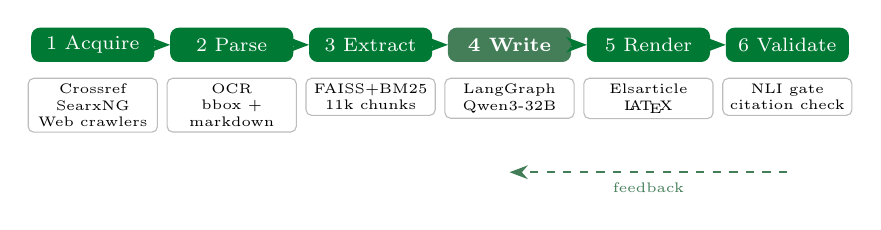
\begin{tikzpicture}[font=\scriptsize,
  stage/.style={draw=ornlgreen,fill=ornlgreen,text=white,rounded corners=3pt,
                minimum height=1.2em,minimum width=1.55cm,inner sep=2pt,align=center},
  sub/.style={draw=ornlgrey!40,fill=white,rounded corners=2pt,
              inner sep=2pt,align=center,font=\tiny,text width=1.50cm,
              text=ornlblack},
  arr/.style={-Stealth,line width=1.0pt,ornlgreen}]
  \node[stage](s1){1 Acquire};
  \node[stage,right=0.20cm of s1](s2){2 Parse};
  \node[stage,right=0.20cm of s2](s3){3 Extract};
  \node[stage,right=0.20cm of s3,fill=backgroundgreen,draw=backgroundgreen](s4){\textbf{4 Write}};
  \node[stage,right=0.20cm of s4](s5){5 Render};
  \node[stage,right=0.20cm of s5](s6){6 Validate};
  \foreach \a/\b in {s1/s2,s2/s3,s3/s4,s4/s5,s5/s6}{\draw[arr](\a)--(\b);}
  \node[sub,below=0.20cm of s1]{Crossref\\SearxNG \\ Web crawlers};
  \node[sub,below=0.20cm of s2]{OCR\\bbox + markdown};
  \node[sub,below=0.20cm of s3]{FAISS+BM25\\11k chunks};
  \node[sub,below=0.20cm of s4]{LangGraph\\Qwen3-32B};
  \node[sub,below=0.20cm of s5]{Elsarticle\\ \LaTeX};
  \node[sub,below=0.20cm of s6]{NLI gate\\citation check};
  \draw[dashed,-Stealth,backgroundgreen,thick]
    ([yshift=-1.4cm]s6.south)--
    node[below,font=\tiny,text=backgroundgreen]{feedback}
    ([yshift=-1.4cm]s4.south);
\end{tikzpicture}\\[2pt]
%% ── Connecting arrow from Stage 4 ──────────────────────────────
{\large\textbf{\color{backgroundgreen}$\Downarrow$ zoom into Stage 4 (Write)}}\\[2pt]
%% ── Bottom: LangGraph 5-agent diagram ──────────────────────────
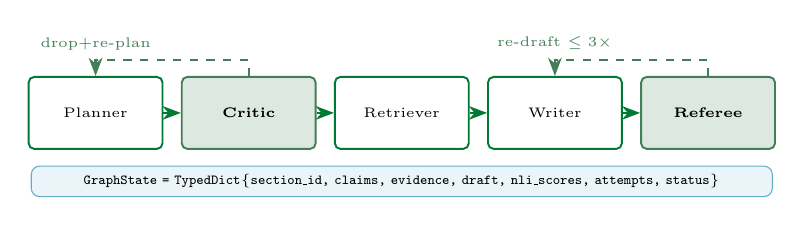
\begin{tikzpicture}[font=\tiny,
  box/.style={draw=ornlgreen,fill=white,rounded corners=2pt,
              minimum height=2.6em,minimum width=1.7cm,
              inner sep=2pt,align=center,text=ornlblack,line width=0.7pt},
  gate/.style={draw=backgroundgreen,fill=backgroundgreen!18,rounded corners=2pt,
               minimum height=2.6em,minimum width=1.7cm,
               inner sep=2pt,align=center,text=ornlblack,
               font=\tiny\bfseries,line width=0.7pt},
  state/.style={draw=cerulean!60,fill=cerulean!8,rounded corners=3pt,
                inner sep=3pt,align=center,text=ornlblack,
                font=\tiny\ttfamily,text width=9.2cm},
  arr/.style={-Stealth,ornlgreen,thick},
  msg/.style={-Stealth,cerulean!70,dashed,thin}]
  \node[box](plan){Planner};
  \node[gate,right=0.22cm of plan](crit){Critic};
  \node[box,right=0.22cm of crit](ret){Retriever};
  \node[box,right=0.22cm of ret](write){Writer};
  \node[gate,right=0.22cm of write](ref){Referee};
  \draw[arr](plan)--(crit);\draw[arr](crit)--(ret);
  \draw[arr](ret)--(write);\draw[arr](write)--(ref);
  \draw[-Stealth,dashed,backgroundgreen,thick]
    (crit.north)--++(0,0.20)-|node[above,font=\tiny]{drop+re-plan}(plan.north);
  \draw[-Stealth,dashed,backgroundgreen,thick]
    (ref.north)--++(0,0.20)-|node[above,font=\tiny]{re-draft $\leq 3\times$}(write.north);
  \node[state,below=0.20cm of ret]{%
    GraphState = TypedDict\{section\_id, claims, evidence, draft,
    nli\_scores, attempts, status\}};
\end{tikzpicture}\\[2pt]
{\scriptsize\color{ornlgreen}\textbf{Why a graph:} The graph breaks broad scientific questions into focused sub-questions, while a shared state records sources and decisions for per-claim traceability.}
\end{frame}

\note{
\tiny

The system operates in six sequential stages, beginning with Acquire, which collects relevant articles from Crossref, uses SearxNG paired with custom web crawlers. \\


The Parse module uses MinerU to convert these PDFs into markdown format , while preserving the original layout and order. \\

The Extract stage then processes this text to build a hybrid retrieval index over thousands of markdown chunks.\\


At the core of the system is the Write stage, a five-agent LangGraph workflow powered by Qwen3.6 35B. \\



Within this stage, a Planner agent first maps out a list of claims to support based on the section specifications. The Critic then evaluates these claims, removing any that lack sufficient evidence before drafting begins. \\


Next, the Retriever agent gathers supporting passages, and the Writer drafts the sections. \\


Finally, the Referee component verifies that the draft is faithful to the retrieved evidence, managing up to three revision cycles before granting final approval.\\

Once drafting is complete, Render compiles the LaTeX . \\

In the final stage, Validate conducts citation verification and natural language inference checks, feeding any detected issues back to the Write stage for automated revision.\\

% interpretation accent first  NLI: Natural Language Interpretation\\
}

%% ═══════════════════════════════════════════════════════════════
%% 4b — (merged into Ontologies slide)
%% ═══════════════════════════════════════════════════════════════
\note{The pipeline starts from a single reference paper. It produces two intermediate files that remain editable: one captures the structure—sections and research questions—and the other captures style, including voice, tense, and rhetorical patterns.}

%% ═══════════════════════════════════════════════════════════════
%% 5 — ONTOLOGY (NEW — replaces OCR image-only)
%% ═══════════════════════════════════════════════════════════════
% \begin{frame}{Ontologies Tell Agents What and How to Write}
% \begin{columns}[T]
%   \begin{column}{0.50\textwidth}
%     \textbf{\color{ornlgreen}Structure ontology} — what to write\\[2pt]
%     {\scriptsize 18 sections extracted from the reference paper:}
%     \begin{center}
%     \begin{tikzpicture}[font=\tiny,
%       sec/.style={draw=ornlgreen,fill=white,rounded corners=2pt,
%                   inner sep=2pt,align=left,text=ornlblack,
%                   minimum width=3.0cm},
%       sub/.style={draw=ornlgreen!50,fill=ornlgreen!5,rounded corners=2pt,
%                   inner sep=2pt,align=left,text=ornlblack,
%                   minimum width=2.6cm},
%       arr/.style={-Stealth,ornlgreen!70,thin}]
%       \node[sec](abs){\textbf{Highlights} \textcolor{ornlgrey}{abstract}};
%       \node[sec,below=0.06cm of abs](s1){\textbf{1. Intro} \textcolor{ornlgrey}{motivation}};
%       \node[sec,below=0.06cm of s1](s2){\textbf{2. T Breeding} \textcolor{ornlgrey}{background}};
%       \node[sub,right=0.20cm of s2,yshift=0.20cm](s21){2.1 Preparations};
%       \node[sub,below=0.04cm of s21](s22){2.2 Mech. Properties};
%       \node[sub,below=0.04cm of s22](s23){2.3 Thermal Props.};
%       \node[sec,below=0.20cm of s2](s3){\textbf{3. Irradiation} \textcolor{ornlgrey}{background}};
%       \node[sec,below=0.06cm of s3](s4){\textbf{4. Advanced} \textcolor{ornlgrey}{discussion}};
%       \node[sec,below=0.06cm of s4](s5){\textbf{5. Gaps} \textcolor{ornlgrey}{gaps}};
%       \node[sec,below=0.06cm of s5](s6){\textbf{6. Conclusions} \textcolor{ornlgrey}{conclusion}};
%       \draw[arr](s2.east)--(s21.west);
%       \draw[arr](s2.east)--(s22.west);
%       \draw[arr](s2.east)--(s23.west);
%     \end{tikzpicture}
%     \end{center}
%     {\scriptsize Each node $\to$ \{role, purpose, expected\_evidence,
%      research\_questions\}.}
%   \end{column}
%   \begin{column}{0.48\textwidth}
%     \textbf{\color{backgroundgreen}Style ontology} — how to write\\[2pt]
%     {\scriptsize\ttfamily voice: passive\\
%      tense: past\\
%      hedging: medium\\
%      citation: numeric}\\[8pt]
%     \textbf{\color{cerulean} Chunk} — what to retrieve\\[2pt]
%     {\scriptsize\ttfamily\textcolor{ornlgreen}{%
%     Material:Li2TiO3\\
%     Property:tritium.T50\\
%     Condition:temp\_K=673\\
%     bbox=[72,310,540,442]}}\\[6pt]
%   \end{column}
% \end{columns}
% \vspace{2pt}
% \begin{itemize}
% \tiny
%     \item \textbf{Planner}: Generates claims from the Structure ontology.
%     \item \textbf{Retriever}: Retrieves evidence using ontology tags.
%     \item \textbf{Writer}: Drafts text under style constraints.
% \end{itemize}


% \end{frame}


\begin{frame}{Ontologies Tell Agents What and How to Write}
\begin{columns}[T]
  \begin{column}{0.50\textwidth}
    \textbf{\color{ornlgreen}Structure ontology}: What to write\\[2pt]
    {\scriptsize 18 sections extracted from the reference paper:}
    \begin{center}
    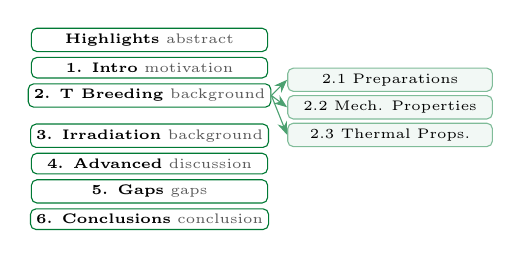
\begin{tikzpicture}[font=\tiny,
      sec/.style={draw=ornlgreen,fill=white,rounded corners=2pt,
                  inner sep=2pt,align=left,text=ornlblack,
                  minimum width=3.0cm},
      sub/.style={draw=ornlgreen!50,fill=ornlgreen!5,rounded corners=2pt,
                  inner sep=2pt,align=left,text=ornlblack,
                  minimum width=2.6cm},
      arr/.style={-Stealth,ornlgreen!70,thin}]
      \node[sec](abs){\textbf{Highlights} \textcolor{ornlgrey}{abstract}};
      \node[sec,below=0.06cm of abs](s1){\textbf{1. Intro} \textcolor{ornlgrey}{motivation}};
      \node[sec,below=0.06cm of s1](s2){\textbf{2. T Breeding} \textcolor{ornlgrey}{background}};
      \node[sub,right=0.20cm of s2,yshift=0.20cm](s21){2.1 Preparations};
      \node[sub,below=0.04cm of s21](s22){2.2 Mech. Properties};
      \node[sub,below=0.04cm of s22](s23){2.3 Thermal Props.};
      \node[sec,below=0.20cm of s2](s3){\textbf{3. Irradiation} \textcolor{ornlgrey}{background}};
      \node[sec,below=0.06cm of s3](s4){\textbf{4. Advanced} \textcolor{ornlgrey}{discussion}};
      \node[sec,below=0.06cm of s4](s5){\textbf{5. Gaps} \textcolor{ornlgrey}{gaps}};
      \node[sec,below=0.06cm of s5](s6){\textbf{6. Conclusions} \textcolor{ornlgrey}{conclusion}};
      \draw[arr](s2.east)--(s21.west);
      \draw[arr](s2.east)--(s22.west);
      \draw[arr](s2.east)--(s23.west);
    \end{tikzpicture}
    \end{center}
    {\scriptsize Each node $\to$ \{role, purpose, expected\_evidence,
     research\_questions\}.}
  \end{column}

  \begin{column}{0.48\textwidth}
    \textbf{\color{backgroundgreen}Style ontology}: How to write\\[2pt]
    {\scriptsize\ttfamily
     % voice: passive\\
     % tense: past\\
     hedging: medium\\
     citation: numeric}\\
    \textbf{\color{cerulean}Indexed Chunk}: What to retrieve\\[2pt]
    {\scriptsize\ttfamily\textcolor{ornlgreen}{%
    Material:Li2TiO3\\
    Property:tritium.T50\\
    Condition:temp\_K=673\\
    bbox=[72,310,540,442]}}\\[6pt]
    %
    % \rule{\linewidth}{0.4pt}\\[3pt]
    {\tiny\textbf{\color{ornlgreen}How both ontologies are produced:}}\\[1pt]
    \centering
    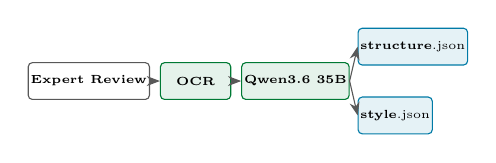
\begin{tikzpicture}[font=\tiny,scale=0.85,transform shape,
      ref/.style={draw=ornlgrey,fill=white,rounded corners=1.5pt,
                  minimum width=1.25cm,minimum height=0.55cm,align=center,
                  text=ornlblack,inner sep=1pt},
      proc/.style={draw=ornlgreen,fill=ornlgreen!10,rounded corners=1.5pt,
                   minimum width=1.05cm,minimum height=0.55cm,align=center,
                   text=ornlblack,inner sep=1pt},
      outbox/.style={draw=cerulean,fill=cerulean!10,rounded corners=1.5pt,
                  minimum width=1.05cm,minimum height=0.55cm,align=center,
                  text=ornlblack,inner sep=1pt},
      arr/.style={-Stealth,ornlgrey,thin}]
      \node[ref](pdf){\textbf{Expert\ Review}};
      \node[proc,right=0.15cm of pdf](mu){\textbf{OCR}};
      \node[proc,right=0.15cm of mu](llm){\textbf{Qwen3.6 35B}};
      \node[outbox,above right=-0.05cm and 0.12cm of llm](sj){\textbf{structure}.json};
      \node[outbox,below right=-0.05cm and 0.12cm of llm](yj){\textbf{style}.json};
      \draw[arr](pdf)--(mu);
      \draw[arr](mu)--(llm);
      \draw[arr](llm.east)--(sj.west);
      \draw[arr](llm.east)--(yj.west);
    \end{tikzpicture}\\[1pt]
    {\tiny\color{ornlgreen}\textbf{Domain expert edits both before any agent runs.}}
  \end{column}
\end{columns}
\end{frame}


\note{

These ontologies act as shared contracts between agents. For example, in selecting lithium solid breeder materials for fusion systems, agents rely on both procedural knowledge (how to navigate design and selection steps) and semantic knowledge (how to interpret material options and properties), both of which can be formalized as ontologies over entities, relations, and constraints.}

% These ontologies serve as the shared contract between agents. Consider an LLM agent tasked with choosing a restaurant: it requires both a map describing how to reach a destination and a map describing the characteristics of possible destinations. The first provides procedural knowledge, while the second provides semantic knowledge. Formally, both maps can be represented as ontologies that define entities, relationships, and constraints within a domain.
% Similarly, generating a literature review requires agents to reason over multiple complementary ontologies. The Structure Ontology tells the Planner what to write by defining section roles, purposes, required evidence, and research questions. The Style Ontology tells the Writer how to write through constraints such as passive voice, past tense, and citation formats. The Chunk Ontology tells the Retriever where to look by organizing evidence according to materials, properties, and experimental conditions. Together, these ontologies provide the shared knowledge representation that enables agents to coordinate planning, retrieval, and writing in a traceable and consistent manner.}

%% ═══════════════════════════════════════════════════════════════
%% 9 — EMBEDDINGS + RESEARCH OUTLINE + QUALITY GATES (merged)
%% ═══════════════════════════════════════════════════════════════
\begin{frame}{Critic and Referee Coverage are Structured Before Writing}


\begin{columns}[T]
  \begin{column}{0.50\textwidth}\centering
    \textbf{\color{ornlgreen}Corpus embedding}\\[2pt]
    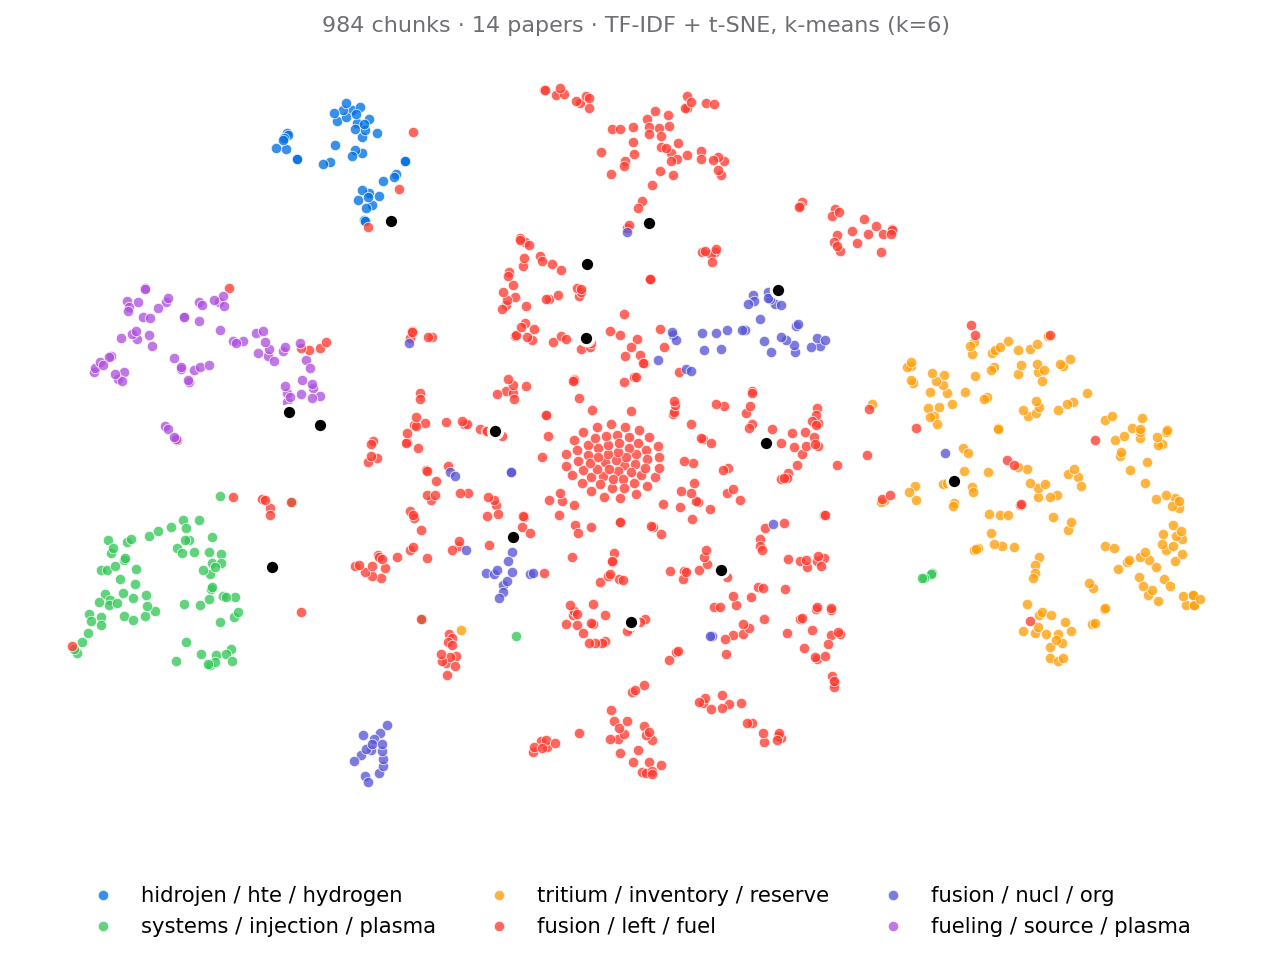
\includegraphics[width=1.2\linewidth]{newfigures/embeddings.png}\\[2pt]
    {\scriptsize\color{ornlgrey} dots = research direction.}
  \end{column}
  \begin{column}{0.58\textwidth}\centering
    \textbf{\color{backgroundgreen}Research-direction outline}\\[2pt]
    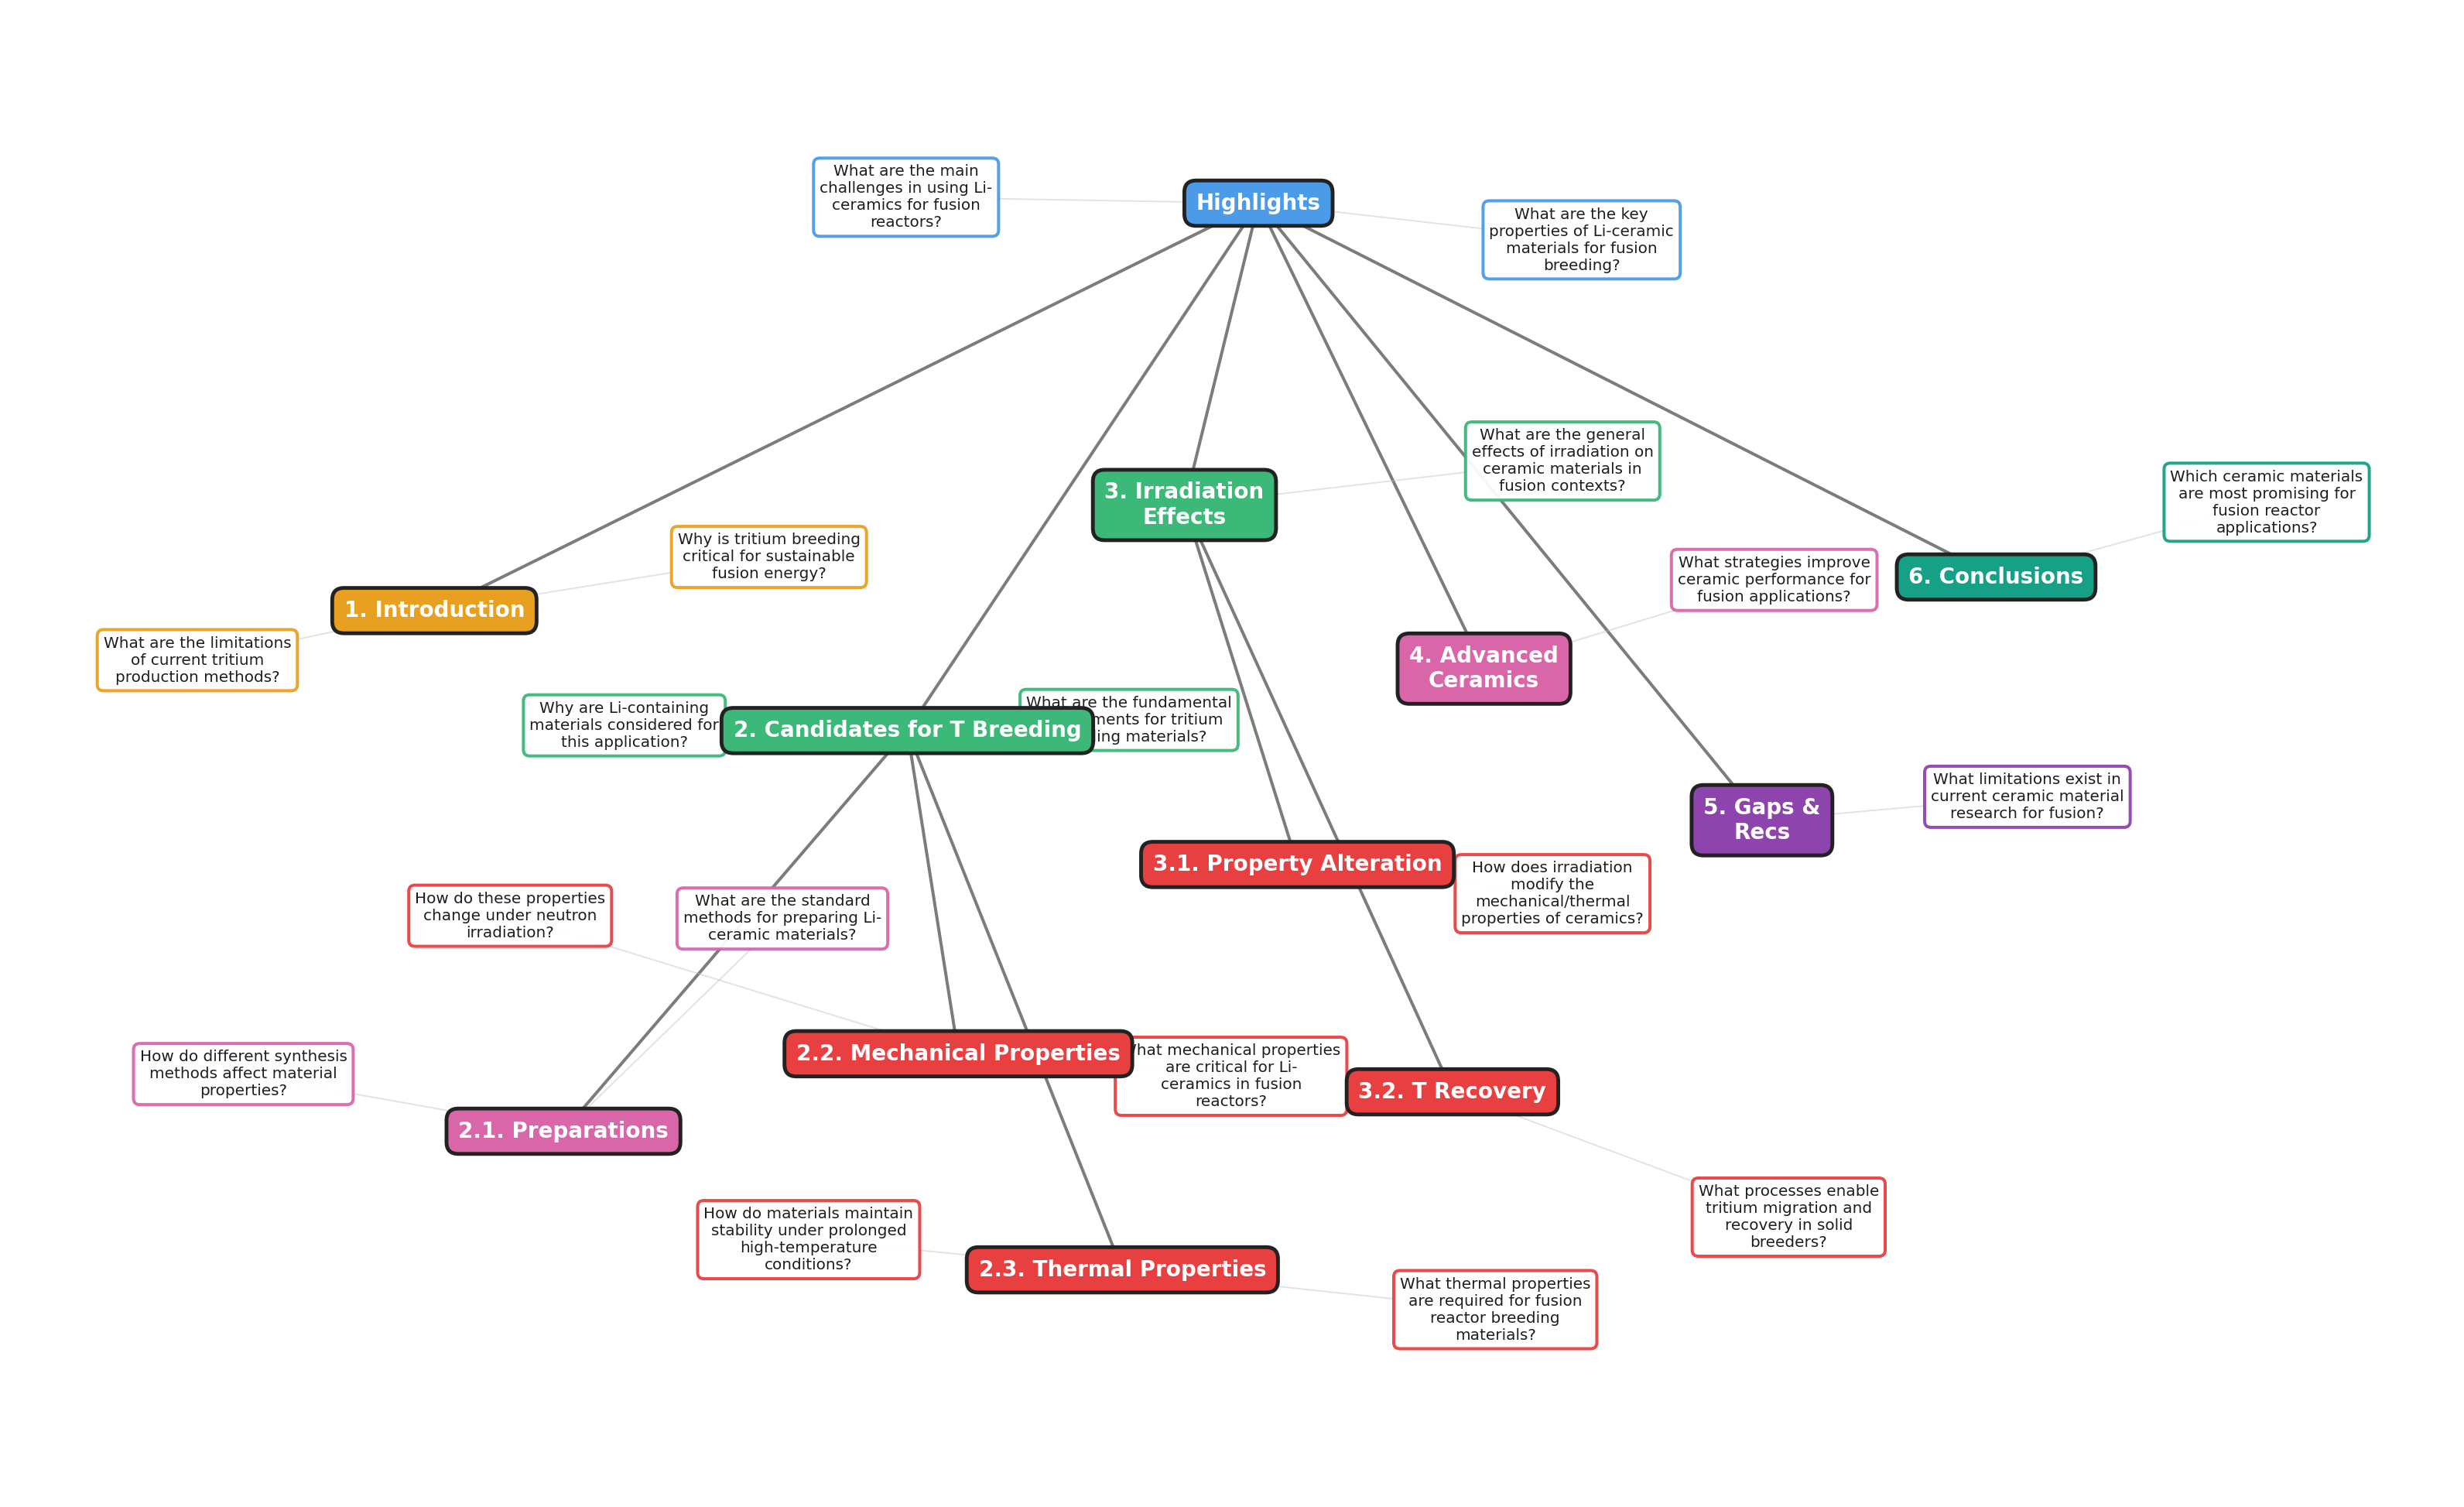
\includegraphics[width=1.2\linewidth]{newfigures/research_directions.png}\\[2pt]
    {\scriptsize\color{ornlgrey}18-section outline extracted from the reference paper.}
  \end{column}
\end{columns}


% \begin{columns}[T]
%   \begin{column}{0.50\textwidth}\centering
%     \textbf{\color{ornlgreen}Corpus embedding}\\[2pt]
%     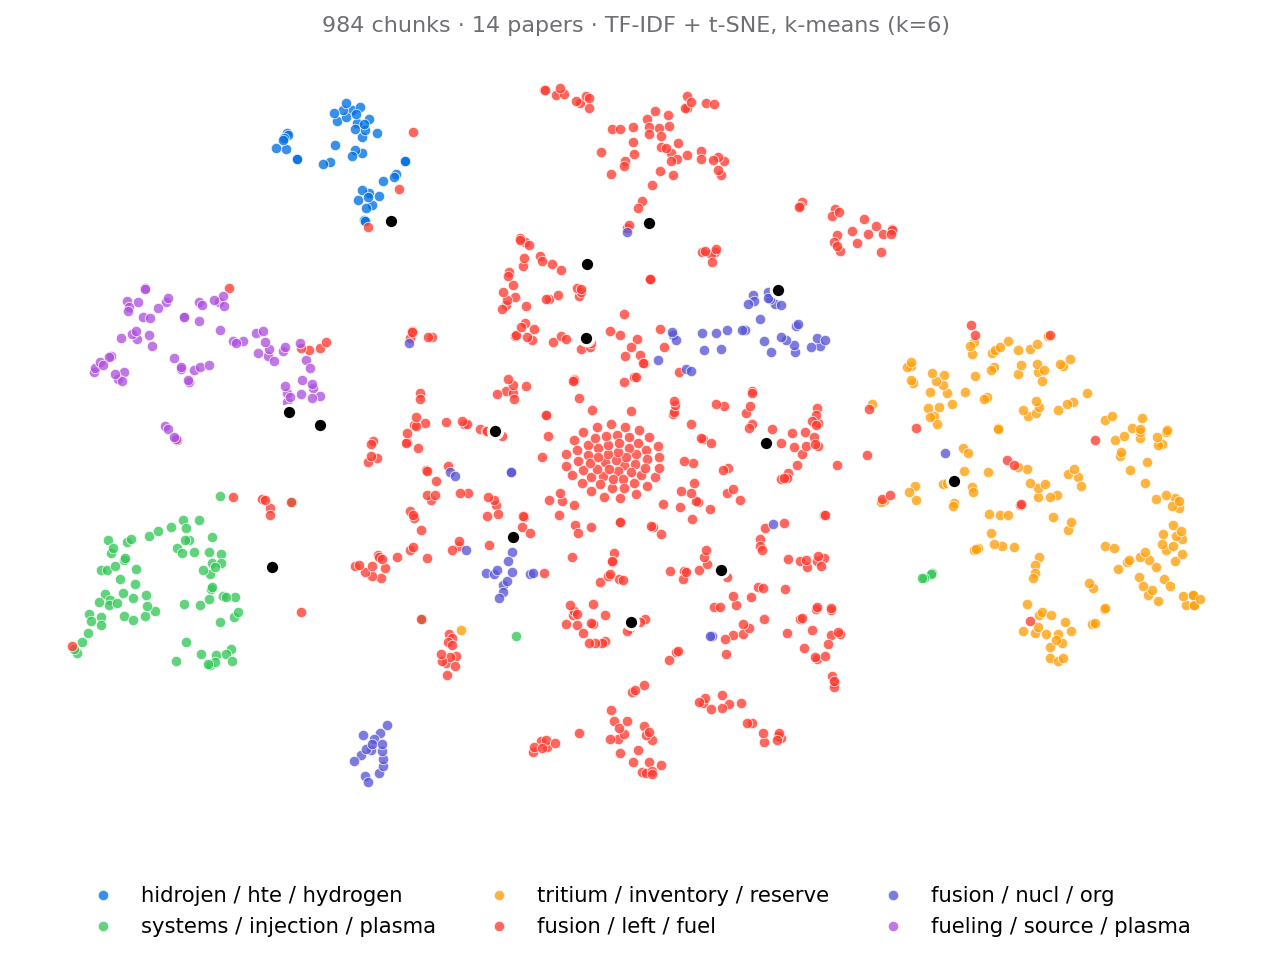
\includegraphics[width=1\linewidth]{newfigures/embeddings.png}\\[2pt]
%     {\scriptsize\color{ornlgrey} black dots = paper centroids.}

%     % TF-IDF\footnote{} $\to$ SVD(50) $\to$ t-SNE; 
%   \end{column}
%   \begin{column}{0.58\textwidth}\centering
%     \textbf{\color{backgroundgreen}Research-direction outline}\\[2pt]
%     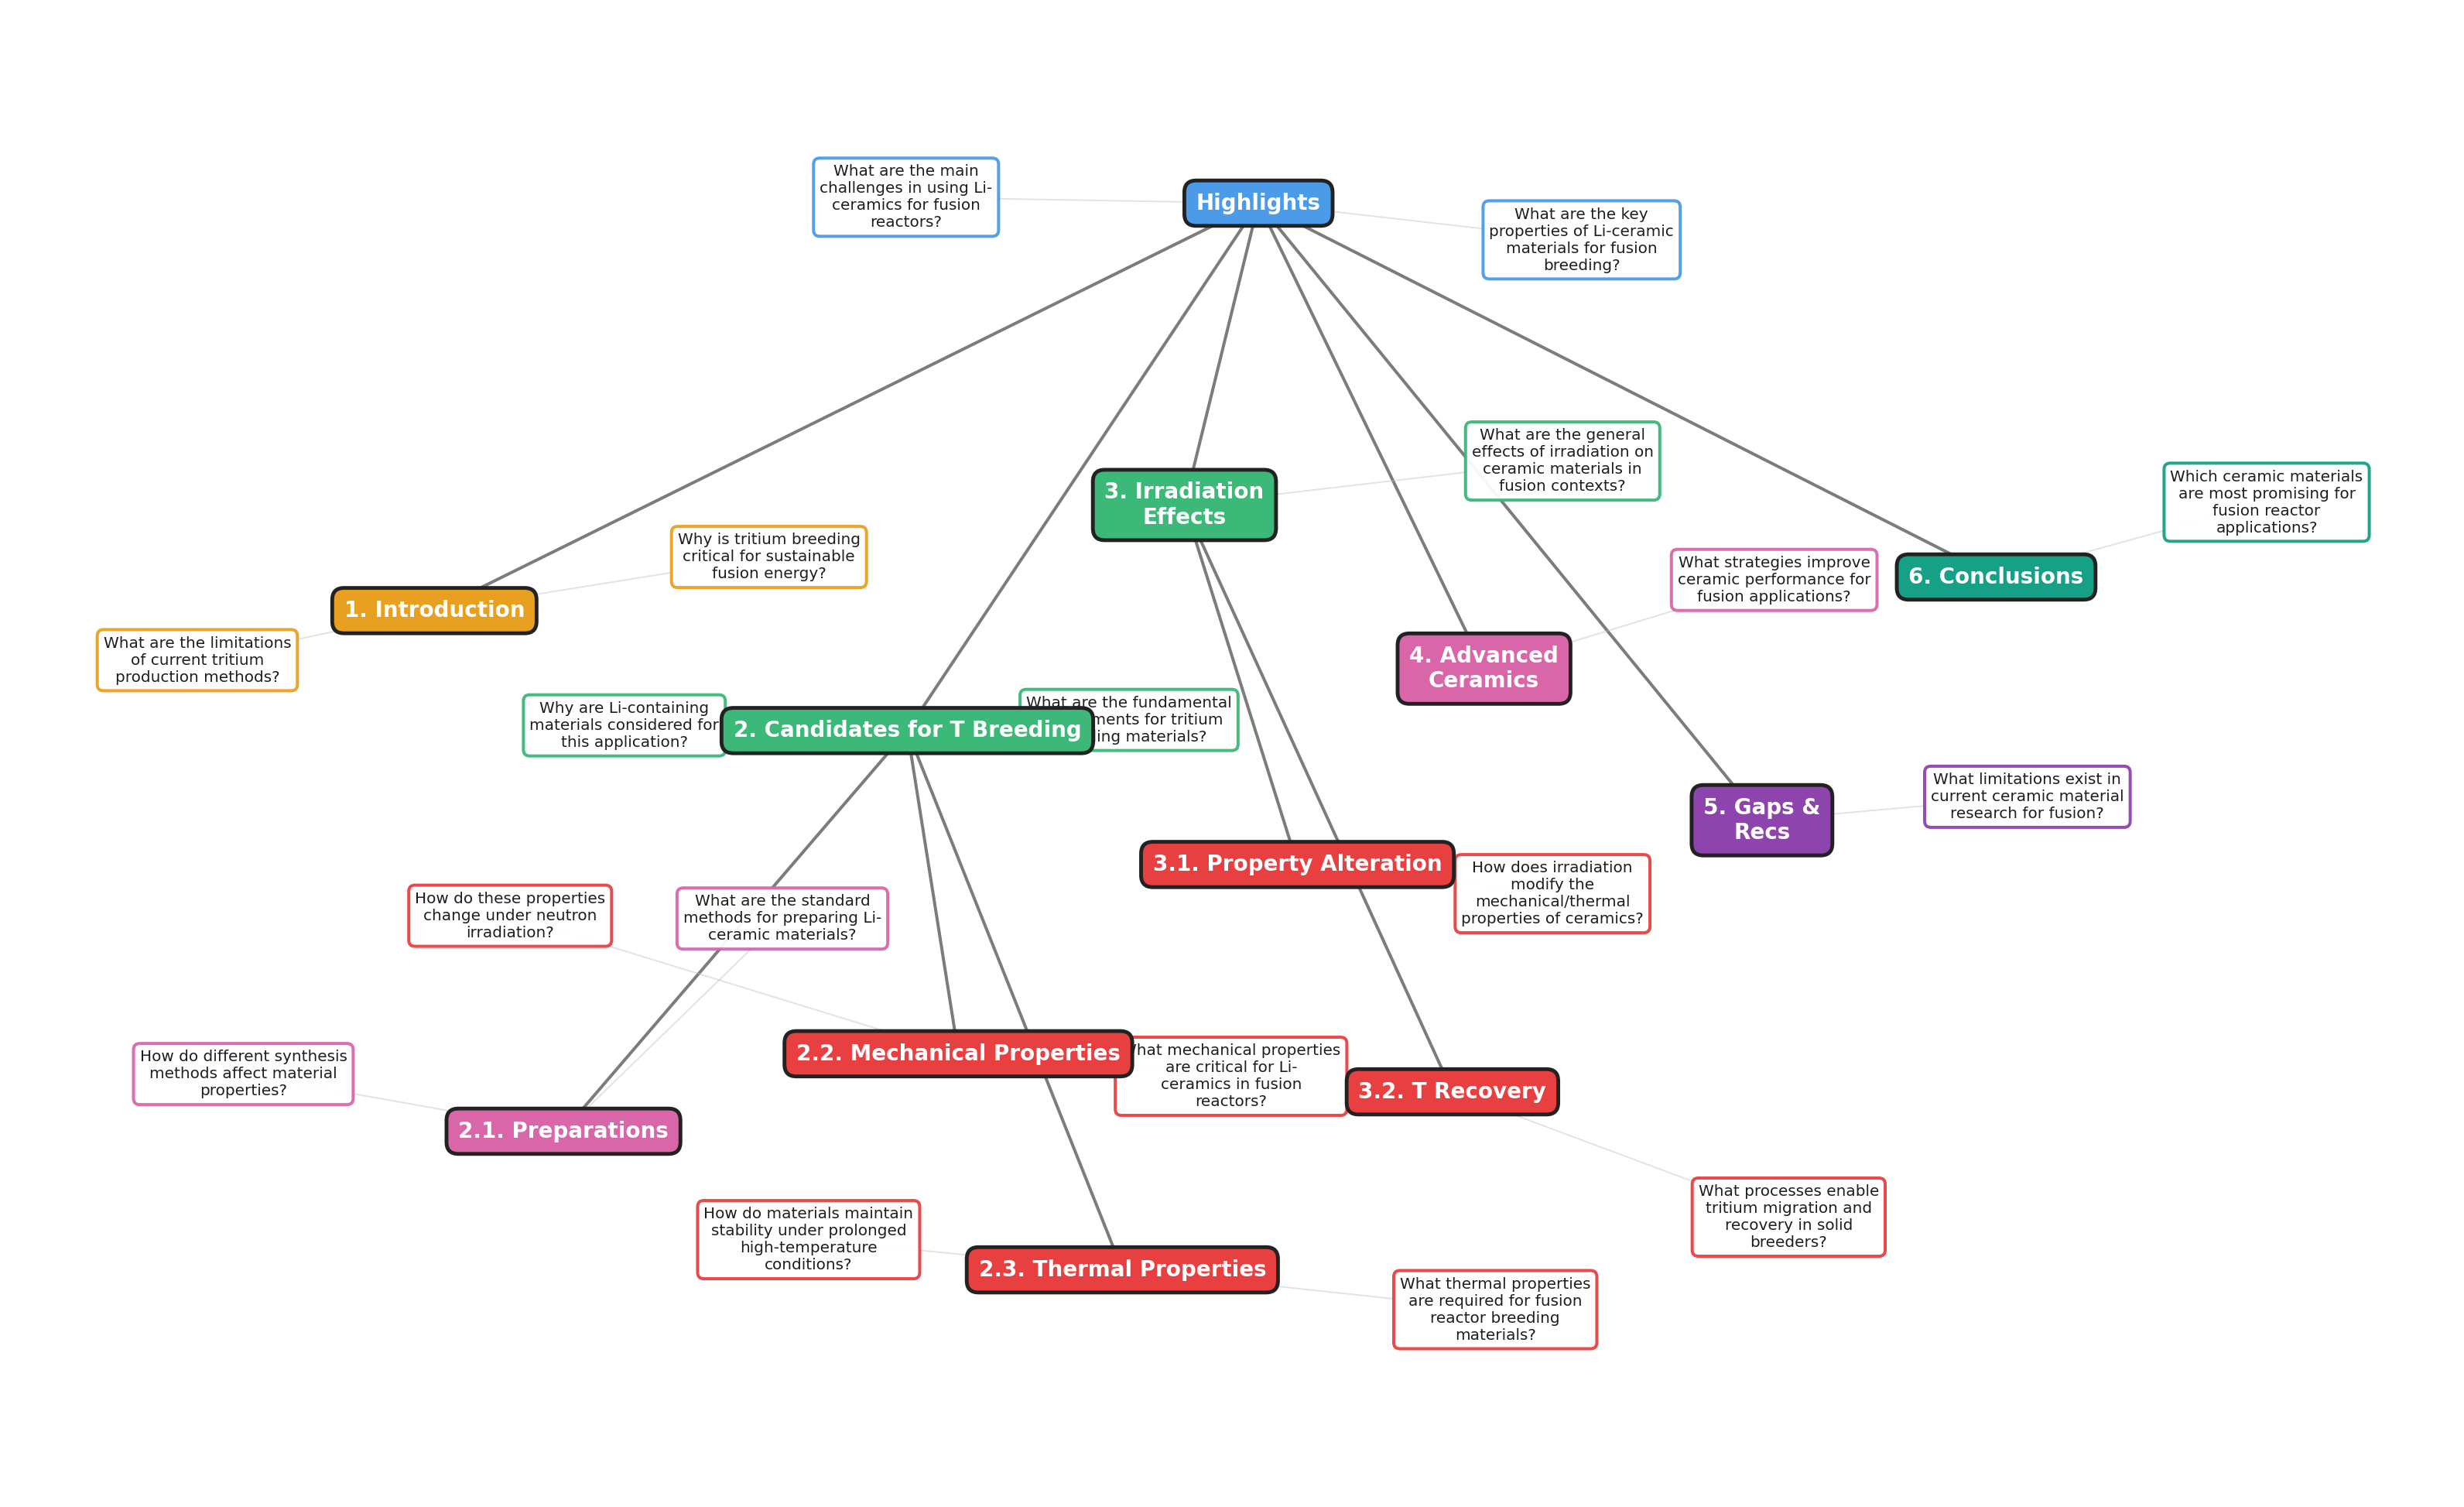
\includegraphics[width=1\linewidth]{newfigures/research_directions.png}\\[2pt]
%     {\scriptsize\color{ornlgrey}18-section outline extracted from the reference paper.}
%   \end{column}
% \end{columns}
% \vspace{4pt}
% \hrule
% \vspace{4pt}
% {\footnotesize
% \textbf{\color{ornlgreen}Critic} (pre-write): $|\mathcal{E}_i|\geq 2$ with distinct sources, else drop.\;\;
% \textbf{\color{backgroundgreen}Referee} (post-write): $P_{\mathrm{ent}}\geq 0.55$ and $|\hat y - y|/|y|\leq 0.10$, else re-draft.\;\;
% \textbf{\color{cerulean}Composite:} $Q = 0.3\,S_g + 0.3\,V_{\mathrm{cite}} + 0.2\,S_f + 0.2\,S_{\mathrm{sty}}$.
% }
\end{frame}
\note{

The Critic rejects claims without at least two supporting chunks. The Referee filters sentences below 0.55 entailment or 10\% numeric error. A final Q score combines grounding, citations, structure, and style.

% The left plot shows our research articles distributed across the relevant topic space using TF-IDF (Term Frequency × Inverse Document Frequency). 


% The Critic blocks any claim with fewer than two distinct supporting chunks before writing. The Referee rejects any sentence that doesn't clear an entailment score of 0.55, or has a numeric deviation above ten percent. The composite Q score then blends grounding, citation validity, structural fidelity, and style alignment.\\

% On the Right side we show the research direction extracted from the ontology


}

%% ═══════════════════════════════════════════════════════════════
%% NEW — PER-CLAIM PAPER SELECTION (hybrid retrieval)
%% ═══════════════════════════════════════════════════════════════
\begin{frame}{Per-Claim Paper Selection: Hybrid Lexical and Semantic Retrieval: Evidence Search}

% Coverage Is Verified Before Any Writing Begins
\centering
\vspace{-2pt}
%% ── top: retrieval flow ──
{\scriptsize
\textbf{\color{ornlgreen}Critic} (pre-write): $|\mathcal{E}_i|\geq 2$ with distinct sources, else drop.\;
\textbf{\color{backgroundgreen}Referee} (post-write): $P_{\mathrm{ent}}\geq 0.55 \wedge |\hat y - y|/|y|\leq 0.10$, else re-draft.\;
\textbf{\color{cerulean}Composite:}\; $Q = 0.3\,S_g + 0.3\,V_{\mathrm{cite}} + 0.2\,S_f + 0.2\,S_{\mathrm{sty}}$.\par}
\vspace{4pt}
%% ── top: retrieval flow ──
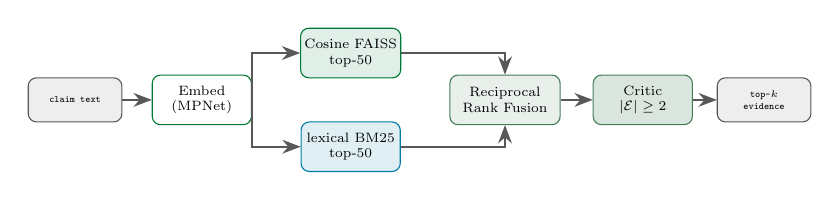
\begin{tikzpicture}[scale=0.70,transform shape,font=\scriptsize,
  box/.style={draw=ornlgreen,fill=white,rounded corners=3pt,
              minimum width=1.8cm,minimum height=0.9cm,align=center,
              text=ornlblack,inner sep=2pt},
  faiss/.style={draw=ornlgreen,fill=ornlgreen!12,rounded corners=3pt,
                minimum width=1.8cm,minimum height=0.9cm,align=center,
                text=ornlblack,inner sep=2pt},
  bm/.style={draw=cerulean,fill=cerulean!12,rounded corners=3pt,
             minimum width=1.8cm,minimum height=0.9cm,align=center,
             text=ornlblack,inner sep=2pt},
  fuse/.style={draw=backgroundgreen,fill=backgroundgreen!12,rounded corners=3pt,
               minimum width=2.0cm,minimum height=0.9cm,align=center,
               text=ornlblack,inner sep=2pt},
  crit/.style={draw=backgroundgreen,fill=backgroundgreen!20,rounded corners=3pt,
               minimum width=1.8cm,minimum height=0.9cm,align=center,
               text=ornlblack,inner sep=2pt},
  data/.style={draw=ornlgrey,fill=ornlgrey!10,rounded corners=3pt,
               minimum width=1.7cm,minimum height=0.8cm,align=center,
               text=ornlblack,inner sep=2pt,font=\tiny\ttfamily},
  arr/.style={-Stealth,ornlgrey,thick}]

  \node[data] (q)    at (0,0)        {claim text};
  \node[box]  (e)    at (2.3,0)      {Embed\\(MPNet)};
  \node[faiss](f)    at (5.0,0.85)   {Cosine FAISS\\top-50};
  \node[bm]   (b)    at (5.0,-0.85)  {lexical BM25\\top-50};
  \node[fuse] (rrf)  at (7.8,0)      {Reciprocal\\Rank Fusion};
  \node[crit] (c)    at (10.3,0)     {Critic\\$|\mathcal{E}|\geq 2$};
  \node[data] (out)  at (12.5,0)     {top-$k$\\evidence};

  \draw[arr] (q)--(e);
  \draw[arr] (e.east)|-(f.west);
  \draw[arr] (e.east)|-(b.west);
  \draw[arr] (f.east)-|(rrf.north);
  \draw[arr] (b.east)-|(rrf.south);
  \draw[arr] (rrf)--(c);
  \draw[arr] (c)--(out);
\end{tikzpicture}\\[9pt]

%% ── bottom: entailment box (col 1) + bar chart (col 2) ──
\vspace{-2pt}
\begin{columns}[T]
  \begin{column}{0.40\textwidth}
    \vspace{4pt}
    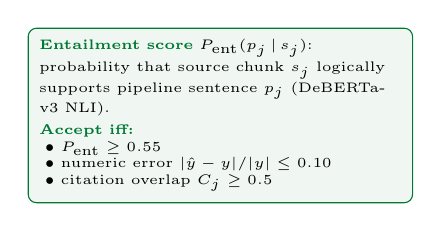
\begin{tikzpicture}
      \node[draw=ornlgreen,fill=ornlgreen!6,rounded corners=3pt,
            inner sep=4pt,text width=4.6cm,align=left,
            text=ornlblack,font=\tiny]{%
        \textbf{\color{ornlgreen}Entailment score} $P_{\mathrm{ent}}(p_j\,|\,s_j)$:\\[1pt]
        probability that source chunk $s_j$ logically supports pipeline sentence $p_j$ (DeBERTa-v3 NLI).\\[2pt]
        \textbf{\color{ornlgreen}Accept iff:}\\
        \;$\bullet$ $P_{\mathrm{ent}}\geq 0.55$\\
        \;$\bullet$ numeric error $|\hat y - y|/|y|\leq 0.10$\\
        \;$\bullet$ citation overlap $C_j\geq 0.5$};
    \end{tikzpicture}
  \end{column}
  \begin{column}{0.58\textwidth}\centering
    {\fontsize{7pt}{8pt}\selectfont\color{ornlgrey}values logged to \texttt{retrieval\_audit.json}}\\[2pt]
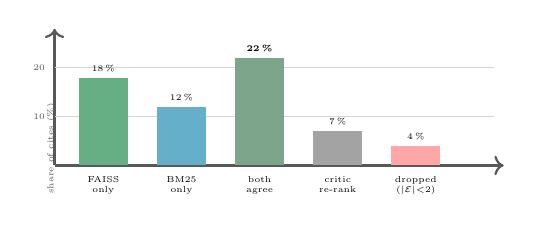
\begin{tikzpicture}[scale=0.62,transform shape,font=\tiny]
  \draw[->,ornlgrey,thick] (0,0) -- (9.2,0);
  \draw[->,ornlgrey,thick] (0,0) -- (0,2.8);
  \node[font=\tiny,rotate=90,text=ornlgrey,left=2pt] at (0,1.4) {share of cites (\%)};
  \foreach \y/\v in {1.0/10,2.0/20}{%
    \draw[ornlgrey!25,thin] (0,\y)--(9.0,\y);
    \node[font=\tiny,text=ornlgrey,left=2pt] at (0,\y) {\v};}
  \fill[ornlgreen!60]      (0.5,0) rectangle (1.5,1.8);
  \fill[cerulean!60]       (2.1,0) rectangle (3.1,1.2);
  \fill[backgroundgreen!70](3.7,0) rectangle (4.7,2.2);
  \fill[ornlgrey!55]       (5.3,0) rectangle (6.3,0.7);
  \fill[red!35]            (6.9,0) rectangle (7.9,0.4);
  \node[font=\tiny,above=0pt] at (1.0,1.8) {18\,\%};
  \node[font=\tiny,above=0pt] at (2.6,1.2) {12\,\%};
  \node[font=\tiny,above=0pt] at (4.2,2.2) {\bfseries 22\,\%};
  \node[font=\tiny,above=0pt] at (5.8,0.7) {7\,\%};
  \node[font=\tiny,above=0pt] at (7.4,0.4) {4\,\%};
  \node[font=\tiny,below=3pt,align=center] at (1.0,0) {FAISS\\only};
  \node[font=\tiny,below=3pt,align=center] at (2.6,0) {BM25\\only};
  \node[font=\tiny,below=3pt,align=center] at (4.2,0) {both\\agree};
  \node[font=\tiny,below=3pt,align=center] at (5.8,0) {critic\\re-rank};
  \node[font=\tiny,below=3pt,align=center] at (7.4,0) {dropped\\($|\mathcal{E}|{<}2$)};
\end{tikzpicture}
  \end{column}
\end{columns}
\end{frame}

\note{Our hybrid approach uses two retrieval methods: BM25, which finds exact keyword matches, and FAISS, which finds semantically similar content. \\


Running both in parallel improves coverage, since each can capture evidence the other may miss. When both point to the same chunks, it increases confidence in the final claim.

% \note{For each claim, FAISS cosine search and BM25 lexical search run in parallel over the eleven thousand chunks, fused using Reciprocal Rank Fusion. The Critic then prunes any claim without at least two distinct supporting chunks. The bar chart shows that the largest single bucket of finally cited chunks — twenty-two percent — came from both retrievers agreeing. That validation of the hybrid approach is why we run both in parallel rather than picking one.

% BM25: ranking function used by full-text search engines (such as Elasticsearch, Apache Lucene, and PostgreSQL)
}



%% ═══════════════════════════════════════════════════════════════
%% 7c — TRACEABILITY IN ACTION — concrete claim examples
%% ═══════════════════════════════════════════════════════════════
\begin{frame}[shrink=25]{Per-Claim Traceability in Action: Accepted Claims are Incorporated. Failed Claims Are Dropped (Referee)}
\centering
\vspace{-4pt}
%% ── TOP: claim table spanning full width ─────────────────────────
\setlength\tabcolsep{3pt}
\renewcommand{\arraystretch}{1.0}
\tiny
\begin{tabular}{@{}p{5.4cm}p{5.4cm}cp{0.9cm}@{}}
\toprule
\textbf{Pipeline claim (with surrounding context)} &
\textbf{Human expert (BNT review, with context)} &
$E$ & \textbf{Source}\\
\midrule
\textcolor{ornlgrey}{\emph{\ldots upon neutron capture,}}
\textcolor{ornlgreen}{Li$_2$TiO$_3$ T release peaks ${\sim}$673\,K}\textcolor{ornlgrey}{\emph{, enabling efficient breeding.}}
& \textcolor{ornlgrey}{\emph{Out-of-pile experiments report}}
\textcolor{ornlblack}{the tritium release peak near 400\,\textdegree{}C}\textcolor{ornlgrey}{\emph{ for Li$_2$TiO$_3$ pebbles.}}
& \textcolor{red!80!black}{\textbf{0.87}} & \texttt{[42]p.3}\\
\addlinespace[2pt]
\textcolor{ornlgrey}{\emph{Microstructure refines:}}
\textcolor{ornlgreen}{grain ${<}1\,\mu$m after 0.1\,dpa}\textcolor{ornlgrey}{\emph{, raising swelling resistance.}}
& \textcolor{ornlgrey}{\emph{Neutron irradiation campaigns show}}
\textcolor{ornlblack}{sub-micron grain refinement above 0.05\,dpa}\textcolor{ornlgrey}{\emph{, consistent with TEM observations.}}
& \textcolor{red!80!black}{\textbf{0.79}} & \texttt{[17]p.7}\\
\addlinespace[2pt]
\textcolor{ornlgrey}{\emph{Thermal conductivity}}
\textcolor{ornlgreen}{$\kappa$ drops 35\,\% at 0.3\,dpa}\textcolor{ornlgrey}{\emph{, limiting heat extraction.}}
& \textcolor{ornlgrey}{\emph{Post-irradiation examination reports a}}
\textcolor{ornlblack}{30--40\,\% reduction in thermal conductivity}\textcolor{ornlgrey}{\emph{ at comparable dose levels.}}
& \textcolor{red!80!black}{\textbf{0.82}} & \texttt{[23]p.12}\\
\addlinespace[2pt]
\textcolor{ornlgrey}{\emph{Claim asserts}}
\textcolor{cerulean}{Li$_2$ZrO$_3$ superior above 900\,\textdegree{}C}\textcolor{ornlgrey}{\emph{ -- no supporting evidence found.}}
& \textcolor{ornlgrey}{\emph{(BNT review discusses Li$_2$ZrO$_3$ stability but reports}}
\textcolor{ornlblack}{no comparative performance above 900\,\textdegree{}C}\textcolor{ornlgrey}{\emph{.)}}
& \textcolor{red!80!black}{\textbf{0.41}} & \textbf{drop}\\
\bottomrule
\end{tabular}\\[2pt]
{\tiny\color{ornlgrey}\textcolor{ornlgreen}{Green}/black: matched claim text; grey italic: surrounding context; \textcolor{red!80!black}{\textbf{red}}: entailment score $E$; last row dropped ($E<0.55$).}\\[4pt]

%% ── BOTTOM: plot + side scores ───────────────────────────────────
\begin{columns}[c]
  \begin{column}{0.70\textwidth}\centering
    \textbf{\color{backgroundgreen}\scriptsize Per-section alignment scores}\\[1pt]
    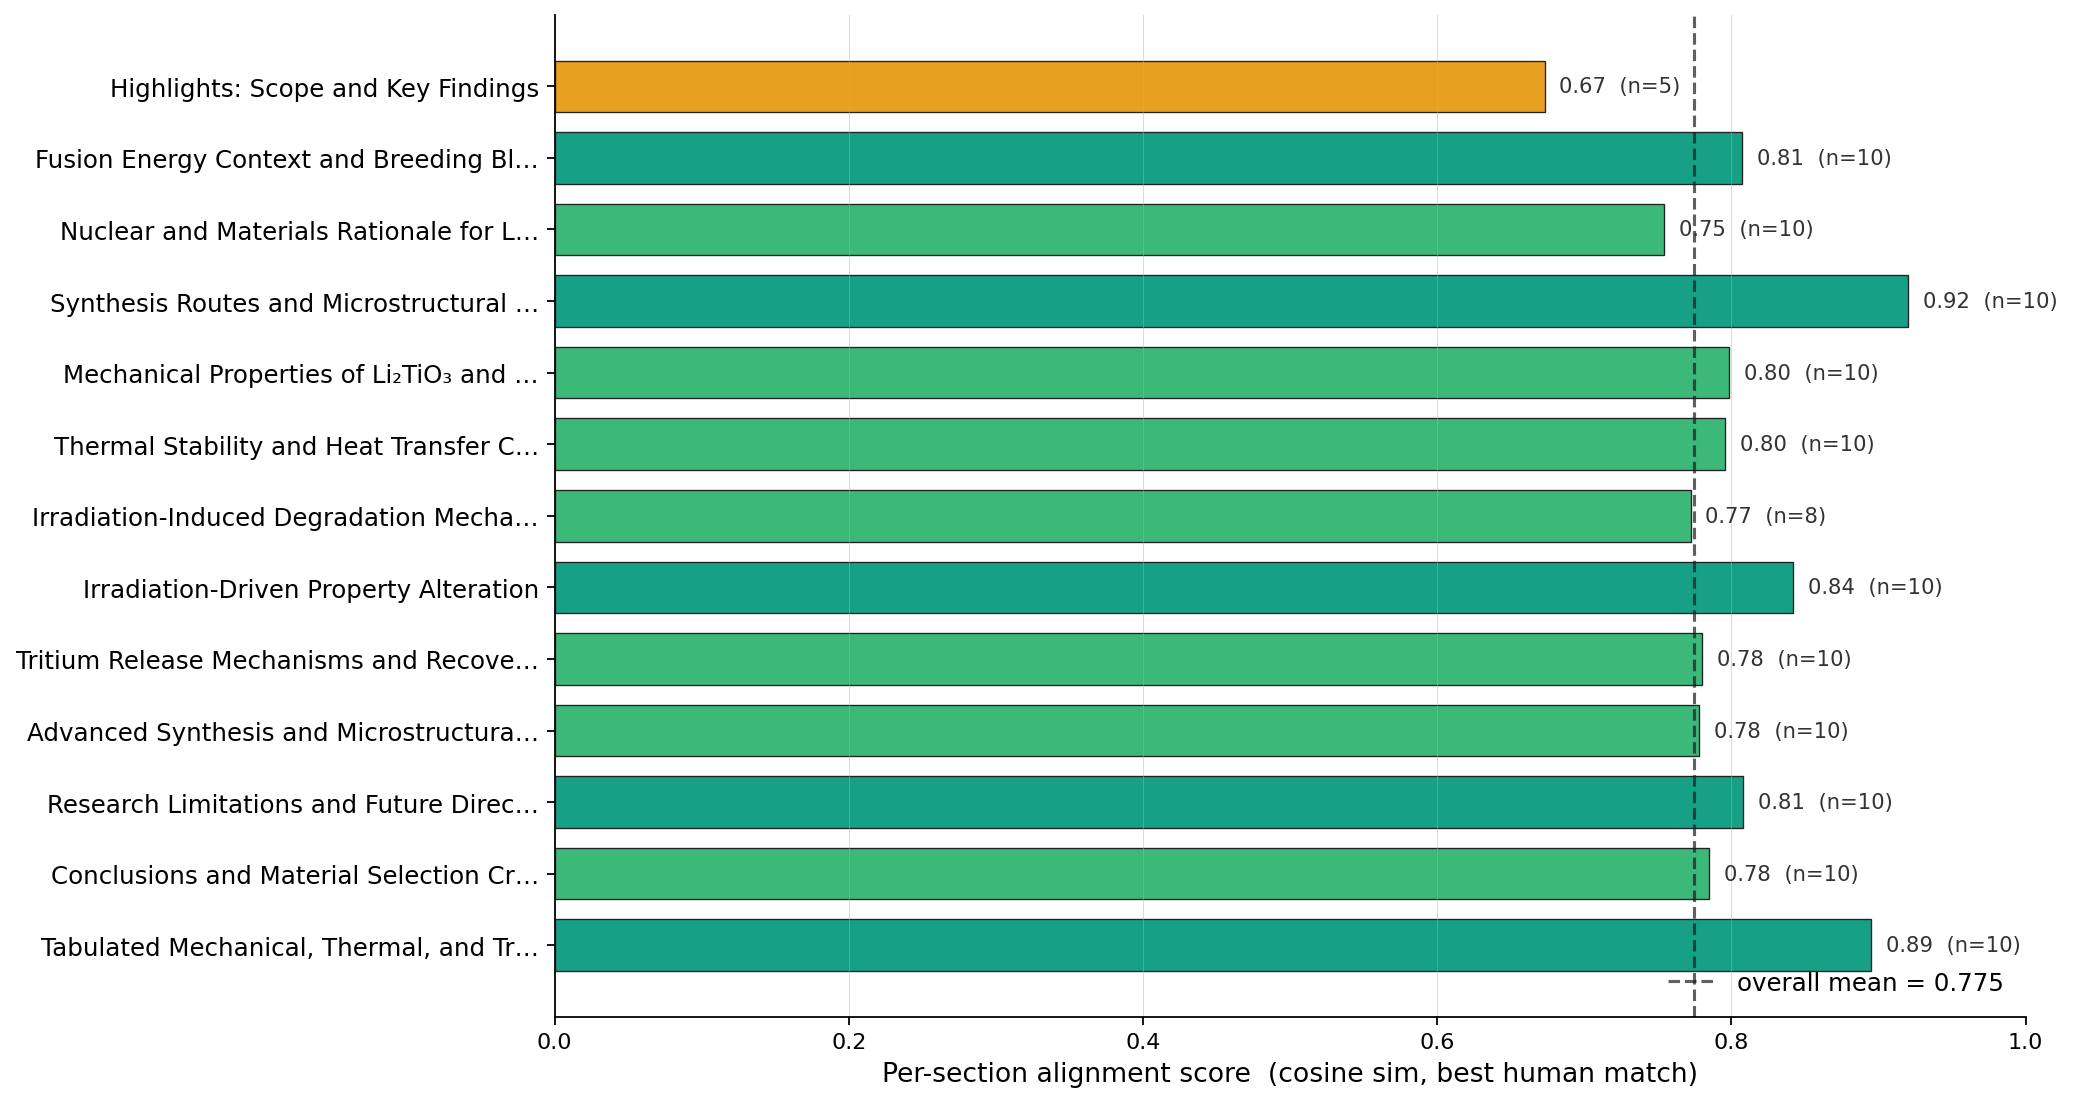
\includegraphics[width=0.95\linewidth,height=2.0cm,keepaspectratio]{newfigures/alignment_per_section.png}
  \end{column}
  \begin{column}{0.29\textwidth}
    \scriptsize
    \setlength\tabcolsep{3pt}
    \renewcommand{\arraystretch}{1.15}
    \begin{tabular}{@{}lr@{}}
    \toprule
    \textbf{Score} & \textbf{Value}\\
    \midrule
    Mean alignment   & \textcolor{ornlgreen}{\textbf{0.77}}\\
    Pairs evaluated  & 167\\
    Accepted ($\geq$\,0.55) & 138\\
    Dropped         & \textcolor{cerulean}{29}\\
    Entailment $E$  & 0.81\\
    % Numeric NMAE    & 0.09\\
    \bottomrule
    \end{tabular}\\[3pt]
    {\tiny\color{ornlgrey}Ground truth: BNT expert review.}\\[4pt]
    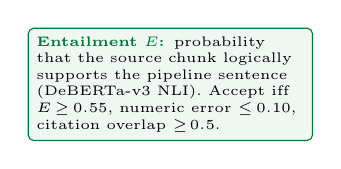
\begin{tikzpicture}
      \node[draw=ornlgreen,fill=ornlgreen!6,rounded corners=2pt,
            inner sep=3pt,text width=3.4cm,align=left,
            text=ornlblack,font=\tiny]{%
        \textbf{\color{ornlgreen}Entailment $E$:} probability that the source chunk logically supports the pipeline sentence (DeBERTa-v3 NLI). Accept iff $E\!\geq\!0.55$, numeric error $\leq\!0.10$, citation overlap $\geq\!0.5$.};
    \end{tikzpicture}
  \end{column}
\end{columns}
\end{frame}
\note{Accepted sentences pass entailment, numeric accuracy, and citation checks, then appear in the manuscript with clickable links to their exact source (paper ID, page, and location).
If a sentence fails any check, it is removed entirely. For example, a claim about lithium zirconate above 900°C was dropped because its entailment score (0.41) was too low.}

%% ═══════════════════════════════════════════════════════════════
%% NEW — SIDE-BY-SIDE: HUMAN EXPERT vs PIPELINE MANUSCRIPT
%% ═══════════════════════════════════════════════════════════════
\begin{frame}{Side-by-Side Comparison: Human and Pipeline Manuscripts Agree on the Same Claims}
\centering
\vspace{-6pt}
\setlength{\fboxsep}{1pt}\setlength{\fboxrule}{1.2pt}
\begin{columns}[T]
  \begin{column}{0.49\textwidth}\centering
    {\small\textbf{\color{ornlgrey}Human-expert manuscript}}\;
    {\tiny\color{ornlgrey}Expert review, p.\,1}\\[2pt]
    \fcolorbox{ornlgrey}{white}{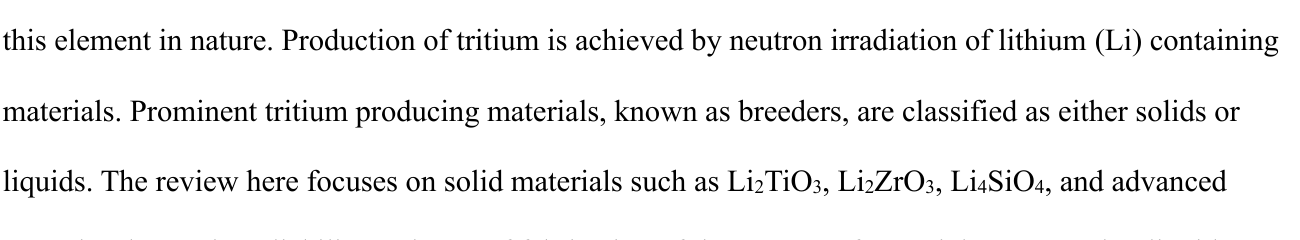
\includegraphics[width=0.93\linewidth]{newfigures/snip_human_1.png}}\\[1pt]
    \fcolorbox{ornlgrey}{white}{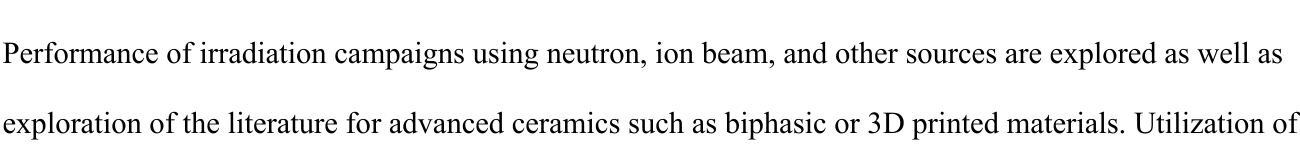
\includegraphics[width=0.93\linewidth]{newfigures/snip_human_2.png}}\\[1pt]
    \fcolorbox{ornlgrey}{white}{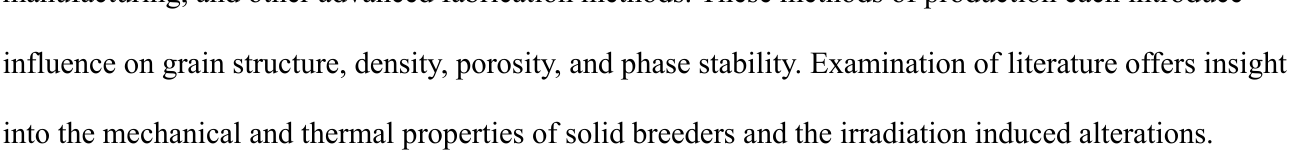
\includegraphics[width=0.93\linewidth]{newfigures/snip_human_3.png}}
  \end{column}
  \begin{column}{0.49\textwidth}\centering
    {\small\textbf{\color{ornlgreen}Pipeline-generated manuscript}}\;
    {\tiny\color{ornlgrey}\texttt{paper.pdf}, p.\,10--11}\\[2pt]
    \fcolorbox{ornlgreen}{white}{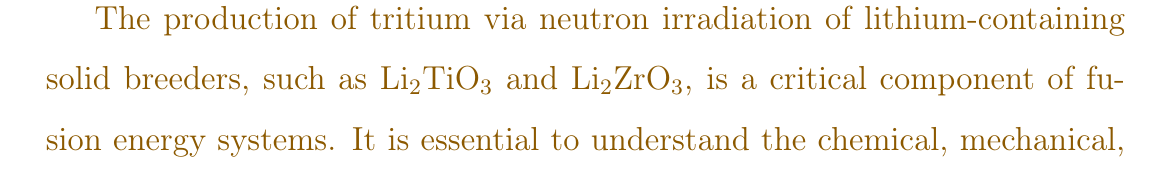
\includegraphics[width=0.93\linewidth]{newfigures/snip_pipe_1.png}}\\[1pt]
    \fcolorbox{ornlgreen}{white}{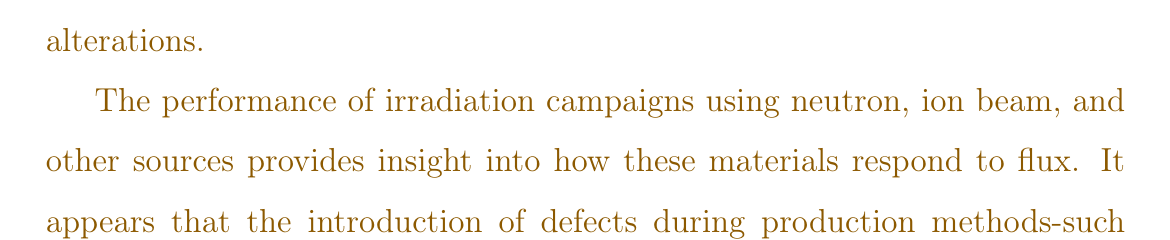
\includegraphics[width=0.93\linewidth]{newfigures/snip_pipe_2.png}}\\[1pt]
    \fcolorbox{ornlgreen}{white}{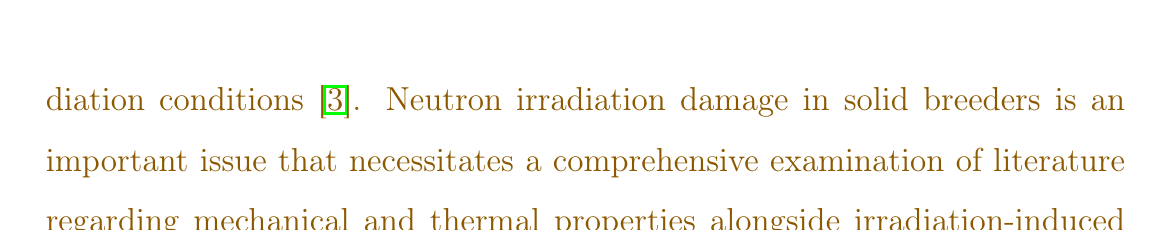
\includegraphics[width=0.93\linewidth]{newfigures/snip_pipe_3.png}}
  \end{column}
\end{columns}
\vspace{2pt}
\begin{center}
\renewcommand{\arraystretch}{0.95}
\setlength\tabcolsep{6pt}
\scriptsize
\begin{tabular}{lc@{\hspace{10pt}}lc@{\hspace{10pt}}lc}\toprule
\textbf{Metric} & \textbf{Score} & \textbf{Metric} & \textbf{Score} & \textbf{Metric} & \textbf{Score}\\\midrule
Claim recall & 0.78 & Faithfulness (NLI) & 0.94 & JSD coverage & 0.12\\
Claim precision & 0.71 & Citation grounding & 1.00 & NMAE numerics & 0.09\\
\multicolumn{4}{r}{\textbf{Composite $Q$}} & \multicolumn{2}{l}{\textbf{0.79}}\\\bottomrule
\end{tabular}
\end{center}
{\tiny\color{ornlgrey}\textit{Irradiation-Driven Property Alteration} \;\textbullet\; pair score \textbf{0.86}}
\end{frame}



%% ═══════════════════════════════════════════════════════════════
%% 10 — DEPLOYMENT (moved up to immediately follow merged slide)
%% ═══════════════════════════════════════════════════════════════
\begin{frame}{The Full Stack Runs Locally on One GPU - One Click Deployment}
\begin{columns}[T]
  \begin{column}{0.42\textwidth}\centering
    % 
\includegraphics[width=0.42\linewidth]{newfigures/docker_logo.png}\\[4pt]
    % 
\includegraphics[width=0.42\linewidth]{newfigures/ollama.png}\\[4pt]

\begin{center}

\includegraphics[height=0.85cm]{newfigures/docker_logo.png}
\hspace{4pt}

\includegraphics[height=0.85cm]{newfigures/ollama.png}

\vspace{2pt}

{\tiny\color{ornlgrey}
Docker containers orchestrate the stack.\\
Ollama serves local LLM inference.\\}
\end{center}

    
    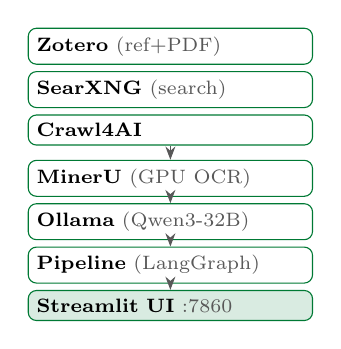
\begin{tikzpicture}[font=\scriptsize,
      cont/.style={draw=ornlgreen,fill=white,rounded corners=3pt,
                   minimum height=1.0em,inner sep=3pt,align=left,
                   text width=3.4cm,text=ornlblack},
      arr/.style={-Stealth,ornlgrey,thin}]
      \node[cont](zot){\textbf{Zotero} \textcolor{ornlgrey}{(ref+PDF)}};
      \node[cont,below=0.08cm of zot](sx){\textbf{SearXNG} \textcolor{ornlgrey}{(search)}};
      \node[cont,below=0.08cm of sx](c4){\textbf{Crawl4AI} \textcolor{ornlgrey}{}};
      \node[cont,below=0.18cm of c4](mu){\textbf{MinerU} \textcolor{ornlgrey}{(GPU OCR)}};
      \node[cont,below=0.08cm of mu](ol){\textbf{Ollama} \textcolor{ornlgrey}{(Qwen3-32B)}};
      \node[cont,below=0.08cm of ol](pg){\textbf{Pipeline} \textcolor{ornlgrey}{(LangGraph)}};
      \node[cont,below=0.08cm of pg,fill=ornlgreen!15](ui){\textbf{Streamlit UI} \textcolor{ornlgrey}{:7860}};
      \draw[arr](c4)--(mu);\draw[arr](mu)--(ol);
      \draw[arr](ol)--(pg);\draw[arr](pg)--(ui);
    \end{tikzpicture}
  \end{column}
  \begin{column}{0.55\textwidth}\centering
    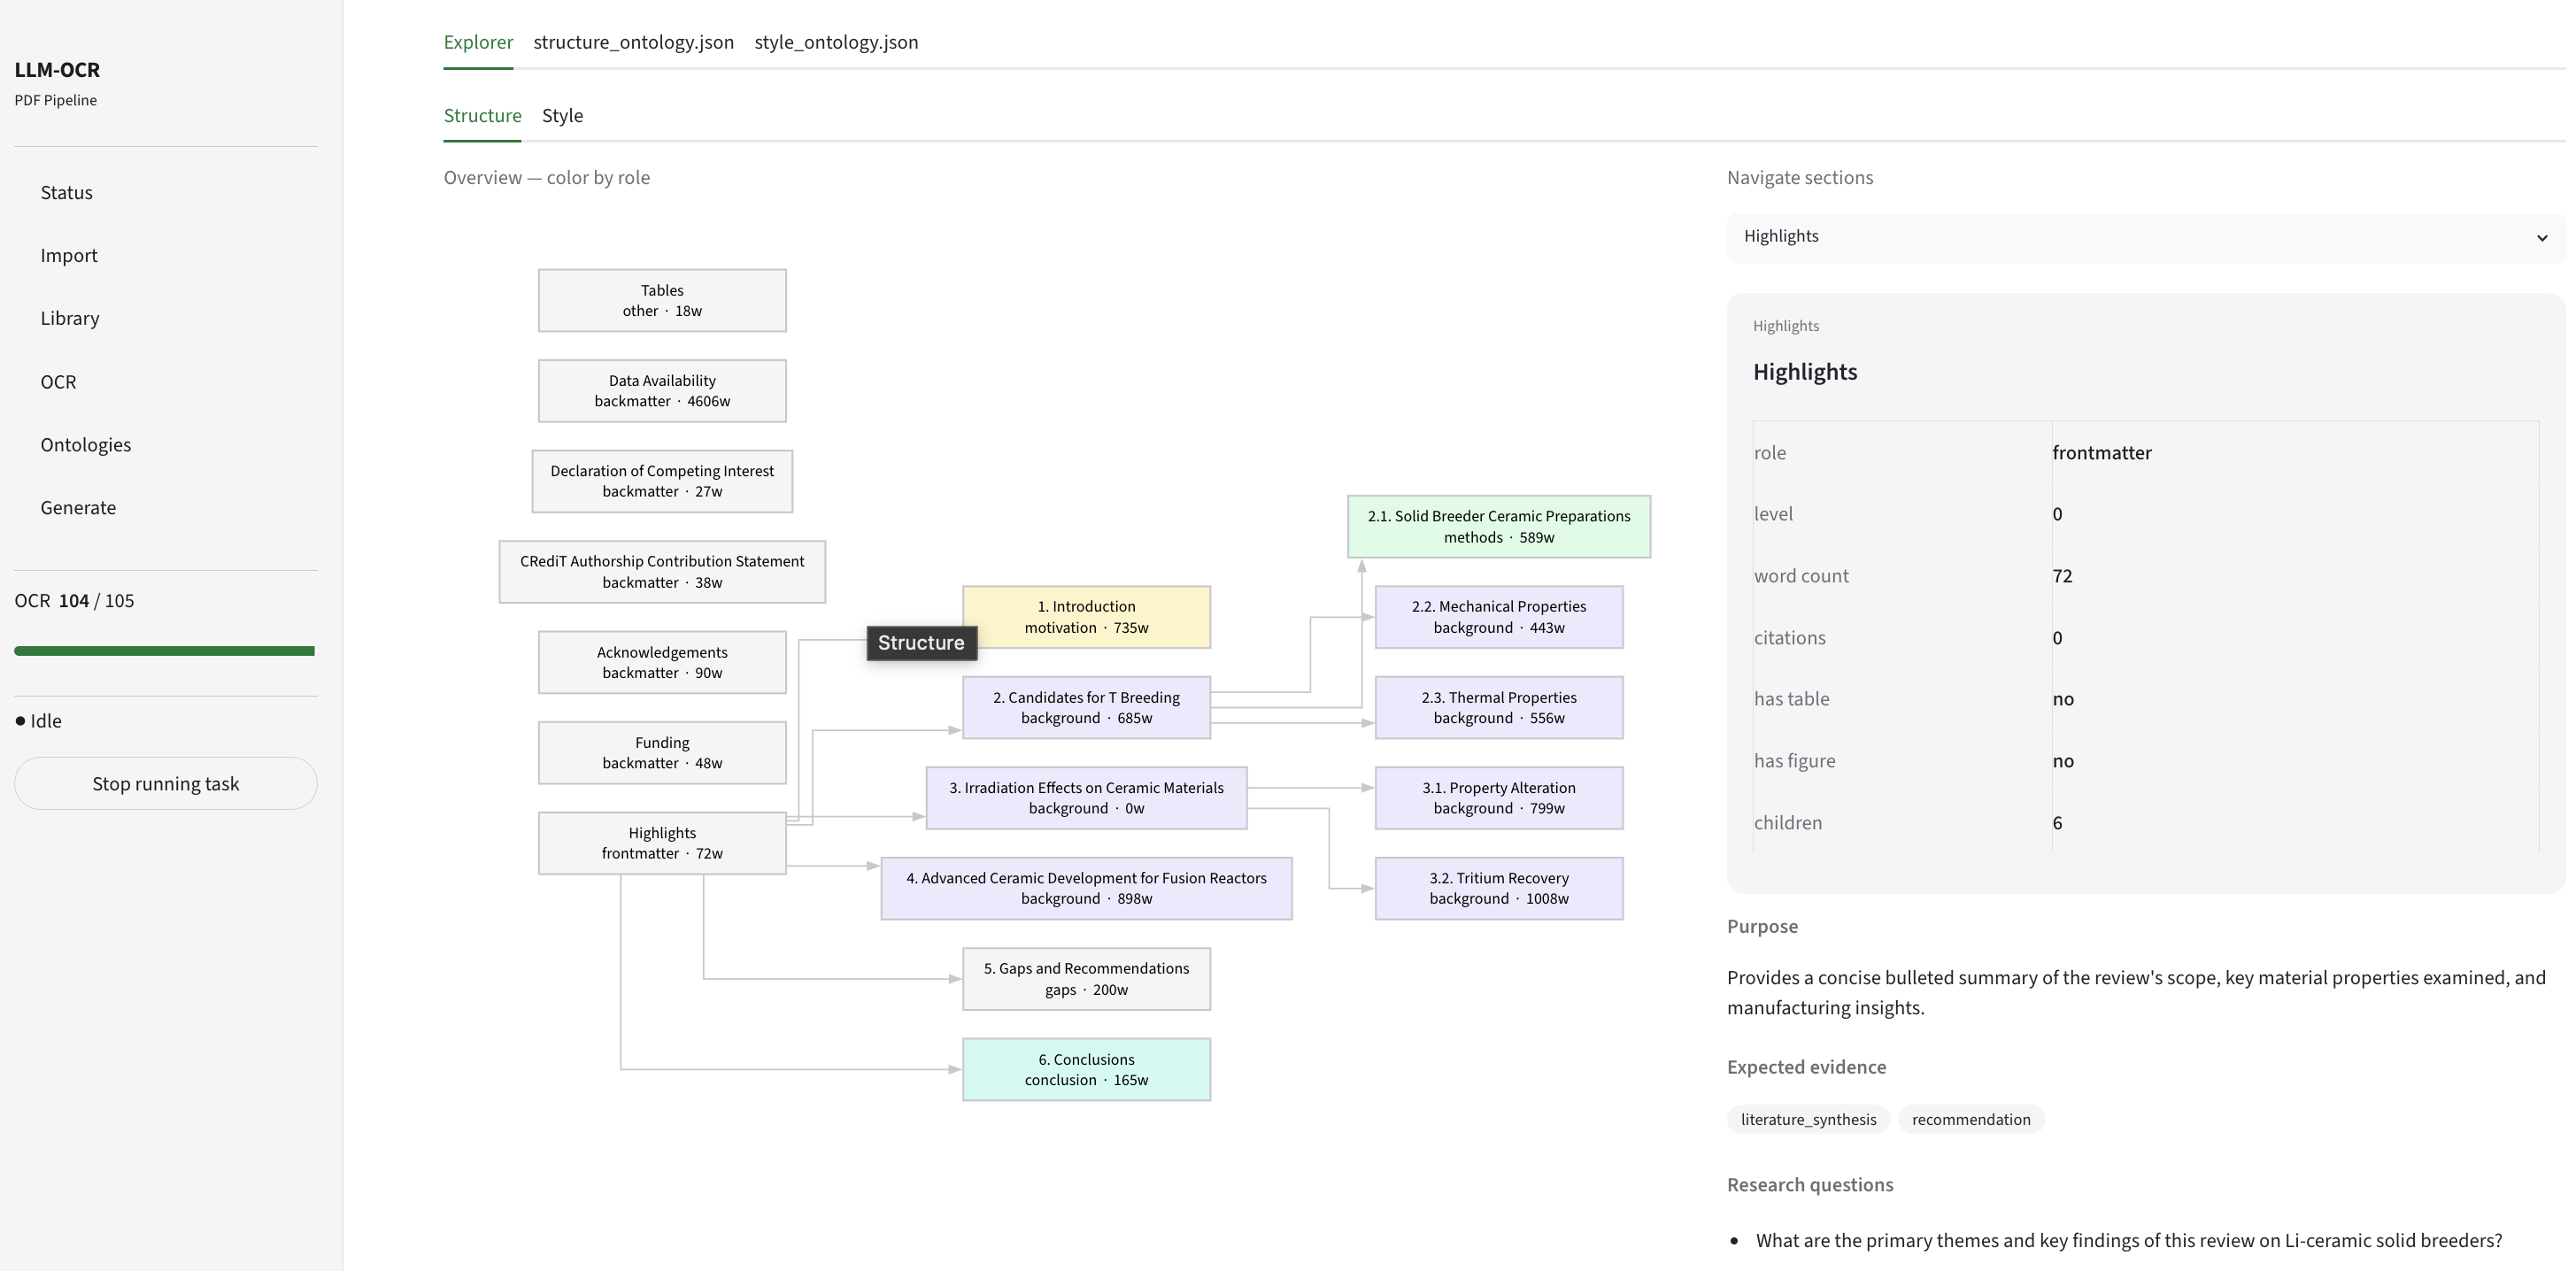
\includegraphics[width=0.98\linewidth]{newfigures/Interface.png}\\[4pt]
    {\scriptsize\color{ornlgrey}Browser interface: Ontology editor, pipeline status, \LaTeX manuscript.}\\[6pt]
    \textbf{\color{ornlgreen}Public images}\\[3pt]
    {\footnotesize
    \;$\bullet$ \textcolor{cerulean}{\href{https://hub.docker.com/r/jtupayac/llm-ocr-pipeline}{hub.docker.com/r/jtupayac/llm-ocr-pipeline}}\\
    \;$\bullet$ \textcolor{cerulean}{\href{https://hub.docker.com/r/jtupayac/llm-ocr-ui}{hub.docker.com/r/jtupayac/llm-ocr-ui}}}
  \end{column}
\end{columns}
\end{frame}
\note{

The whole system runs fully on a single 48GB GPU, The system is sandboxed so no data ever leaves the machine. \\

Setup is quick: just two Docker pulls and one command. It launches all the neccessary tools and packages.\\

Now I’ll open the live interface.\\


[CLICK — wait ~20 seconds]


The interface has three parts: a top outline tree where you can edit nodes like roles, questions, and evidence; a middle panel showing the live agent workflow; and a bottom PDF preview that updates in real time. Everything runs in one browser tab—no coding needed.

}



%% ═══════════════════════════════════════════════════════════════
%% QUESTIONS
%% ═══════════════════════════════════════════════════════════════
{\setbeamertemplate{footline}{}
\begin{frame}[plain]
\centering
\vspace{0.6cm}
{\fontsize{60pt}{72pt}\selectfont\color{ornlgreen}\bfseries Questions?}\\[18pt]
% {\Large\color{ornlblack}Thank you --- happy to discuss.}\\[28pt]
% \begin{tikzpicture}
%   \node[draw=ornlgreen,fill=ornlgreen!8,rounded corners=4pt,
%         inner sep=10pt,align=center,text width=10cm]{%
%     {\large\color{ornlblack}\textbf{Jose Tupayachi}}\\[3pt]
%     {\small\color{ornlgrey}Oak Ridge National Laboratory}\\[6pt]
%     {\normalsize\href{mailto:tupayachij@ornl.gov}{\color{cerulean}\texttt{tupayachij@ornl.gov}}}\\[2pt]
%     {\footnotesize\color{ornlgrey}Co-authors: Gabe Parker, Xueping Li, Xiao-Ying Yu}
%   };
% \end{tikzpicture}
\end{frame}}
\note{Q\&A.}
\note{Here is a side-by-side. The human expert writes a sentence on irradiation-driven property alteration. The pipeline independently generates the same claim, anchored to a specific bounding box in the source manuscript. We show an alignment score: 0.86.}

% %% ═══════════════════════════════════════════════════════════════
% %% FINAL — RESULTS + UI + CONCLUSIONS (merged)
% %% ═══════════════════════════════════════════════════════════════
% \begin{frame}[shrink=18]{Metrics and Validation Scores: Human-Expert Review Against Pipeline Generation}
% \begin{columns}[T]
%   \begin{column}{0.38\textwidth}
%     \textbf{Pipeline results}\\[3pt]
%     \renewcommand{\arraystretch}{1.0}
%     \scriptsize

%     % \textbf{Demonstrated}\\[3pt]
%     % \footnotesize
%     % \begin{itemize}\setlength\itemsep{2pt}
%     %   \item First traceable LLM review for fusion breeders
%     %   \item $Q{=}0.79$ (F\,$=$\,0.94, G\,$=$\,1.00)
%     %   \item 6 months $\to$ 6 hours
%     %   \item Zero hallucinated citations
%     % \end{itemize}
%     \vspace{6pt}
%     % {\scriptsize\color{ornlgrey}%
%     % ORNL/UT-Battelle, DOE DE-AC05-00OR22725.}
%   \end{column}
%   \begin{column}{0.60\textwidth}\centering
%     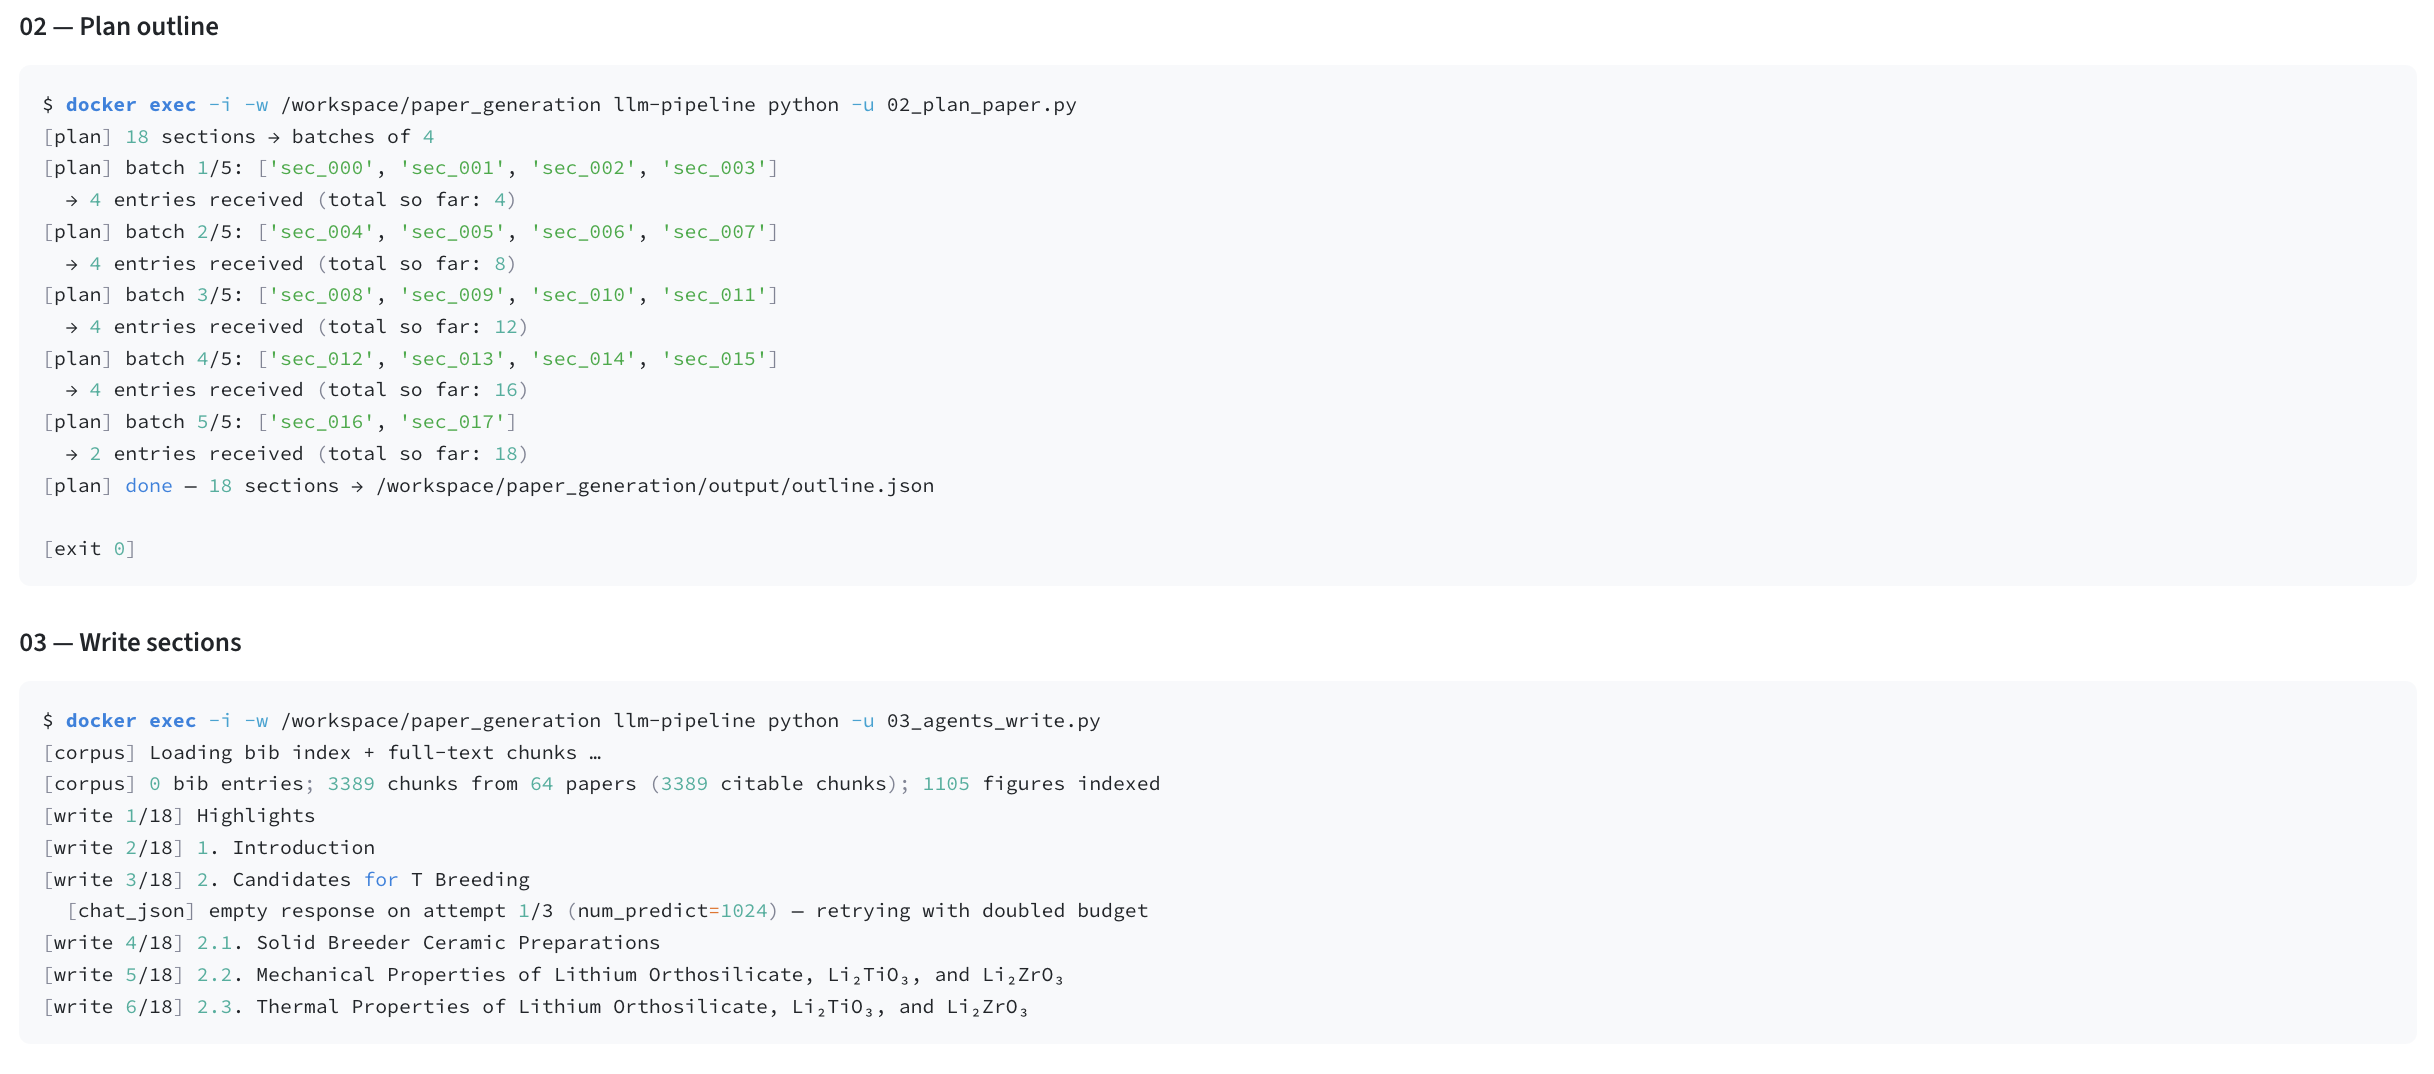
\includegraphics[width=0.96\linewidth]{newfigures/execution.png}\\[3pt]
%     {\scriptsize\color{ornlgrey}Live UI: outline tree (top), agent flow (middle), generated PDF (bottom).}\\[5pt]
%     \footnotesize
%     \begin{itemize}\setlength\itemsep{1pt}
%       \item Click any node $\to$ edit role, RQs, evidence types inline.
%       \item \textbf{Agent flow}, \textbf{corpus embedding}, \textbf{citation network} panels.
%       \item {\textcolor{ornlgreen}{\textbf{No code:}}} edit $\to$ inspect $\to$ generate, in one browser tab.
%     \end{itemize}
%   \end{column}
% \end{columns}
% \end{frame}
% \note{The numbers: claim recall 0.78, precision 0.71, faithfulness 0.94, and citation grounding 1.00 — every single cited value has a verified bounding box in the source document. Composite Q of 0.79.\\

% This is the first traceable LLM-generated review applied to fusion breeder materials. \\

% And the same recipe transfers directly to structural alloys, plasma-facing materials — you can swap the ontology and the retrieval index, leaving the  pipeline runs unchanged.\\


% Thank you.\\

% I'm happy to take questions.\\

% }


% {\setbeamertemplate{footline}{}
% \begin{frame}[plain]
% \centering
% \vspace{0.6cm}
% {\fontsize{60pt}{72pt}\selectfont\color{ornlgreen}\bfseries Questions?}\\[18pt]
% % {\Large\color{ornlblack}Thank you --- happy to discuss.}\\[28pt]
% % \begin{tikzpicture}
% %   \node[draw=ornlgreen,fill=ornlgreen!8,rounded corners=4pt,
% %         inner sep=10pt,align=center,text width=10cm]{%
% %     {\large\color{ornlblack}\textbf{Jose Tupayachi}}\\[3pt]
% %     {\small\color{ornlgrey}Oak Ridge National Laboratory \,/\, University of Tennessee, Knoxville}\\[6pt]
% %     {\normalsize\href{mailto:tupayachij@ornl.gov}{\color{cerulean}\texttt{tupayachij@ornl.gov}}}\\[2pt]
% %     {\footnotesize\color{ornlgrey}Co-authors: Gabe Parker, Xueping Li, Xiao-Ying Yu}
% %   };
% % \end{tikzpicture}
% \end{frame}}
% \note{Q\&A slide. Contact email displayed for follow-up. Backup slides with formal metric definitions and a full glossary follow.}



%% ═══════════════════════════════════════════════════════════════
%% BACKUP — METRICS FORMALLY DEFINED (grayed)
%% ═══════════════════════════════════════════════════════════════
\appendix

\begin{frame}{Backup: Validation Metrics}
\color{ornlgrey!90}
\scriptsize
\renewcommand{\arraystretch}{1.3}
\setlength\tabcolsep{4pt}
\begin{columns}[T]
  %% ── Left: formal definitions ───────────────────────────────────
  \begin{column}{0.56\textwidth}
    \textbf{Formal definitions}\\[3pt]
    \begin{tabular}{@{}p{2.2cm}p{5.4cm}@{}}
    \toprule
    \textbf{Metric} & \textbf{Formula}\\
    \midrule
    Claim recall &
      $R = \dfrac{|\mathcal{C}_h \cap \mathcal{C}_p|}{|\mathcal{C}_h|}$\\[6pt]
    Claim precision &
      $P = \dfrac{|\mathcal{C}_h \cap \mathcal{C}_p|}{|\mathcal{C}_p|}$\\[6pt]
    Faithfulness (NLI) &
      $F = \dfrac{1}{n}\displaystyle\sum_{j} P_{\text{ent}}(p_j \mid s_j)$\\[6pt]
    Citation grounding &
      $G = \dfrac{|\{j : \text{bbox}_j \text{ verified}\}|}{|\mathcal{C}_p|}$\\[6pt]
    Topic divergence &
      $\text{JSD}(H \,\Vert\, P)$ over LDA topic mixtures\\[2pt]
    Numeric error &
      $\text{NMAE} = \dfrac{1}{n}\displaystyle\sum_{j}\dfrac{|\hat y_j - y_j|}{|y_j|}$\\[6pt]
    Composite quality &
      $Q = 0.3\,S_g + 0.3\,V_{\text{cite}} + 0.2\,S_f + 0.2\,S_{\text{sty}}$\\
    \bottomrule
    \end{tabular}
  \end{column}
  %% ── Right: plain-language summaries ────────────────────────────
  \begin{column}{0.42\textwidth}
    \textbf{In plain language}\\[3pt]
    \begin{tabular}{@{}p{2.2cm}p{3.8cm}@{}}
    \toprule
    \textbf{Metric} & \textbf{In five words}\\
    \midrule
    Claim recall      & human facts we recover\\[2pt]
    Claim precision   & our facts matching the human\\[2pt]
    Faithfulness      & sentences supported by source chunk\\[2pt]
    Citation grounding& claims with verified source bbox\\[2pt]
    Topic divergence  & divergence of topic emphasis\\[2pt]
    Numeric error     & mean normalized numeric deviation\\[2pt]
    Composite $Q$     & weighted average of all metrics\\
    \bottomrule
    \end{tabular}\\[6pt]
    {\tiny\color{ornlgrey}
    \textbf{Notation.} $\mathcal{C}_h$, $\mathcal{C}_p$: human and pipeline claim sets. $p_j$, $s_j$: pipeline sentence and source chunk. $P_{\text{ent}}$: DeBERTa-v3-MNLI entailment probability. Accept iff $P_{\text{ent}}{\geq}0.55 \wedge \text{NMAE}{\leq}0.10 \wedge C_j{\geq}0.5$.
    }
  \end{column}
\end{columns}
\end{frame}
\note{Additional Definitions}

\begin{frame}[shrink=55]{Backup: Glossary of Acronyms, Models and Domain Terms Used Throughout the Talk}
\color{ornlgrey!90}
\centering
\footnotesize
\setlength\tabcolsep{5pt}
\renewcommand{\arraystretch}{1.25}
\begin{columns}[T]
  \begin{column}{0.49\textwidth}\centering
    \textbf{Methods and models}\\[2pt]
    \begin{tabular}{@{}p{1.7cm}p{5.6cm}@{}}
    \toprule
    \textbf{Term} & \textbf{Meaning}\\
    \midrule
    TF-IDF    & Term Frequency $\times$ Inverse Document Frequency.\\
    SVD       & Singular Value Decomposition (TF-IDF $\to$ 50 dims).\\
    t-SNE     & t-Distributed Stochastic Neighbor Embedding (2D vis).\\
    LDA       & Latent Dirichlet Allocation; topic-mixture model.\\
    BM25      & Okapi BM25 lexical relevance score.\\
    FAISS     & Facebook AI Similarity Search; dense vector index.\\
    MPNet     & Masked-and-Permuted sentence-embedding transformer.\\
    RRF       & Reciprocal Rank Fusion of multiple rankings.\\
    NLI       & Natural Language Inference; entailment classifier.\\
    LangGraph & Typed-state agent-graph framework on LangChain.\\
    MinerU    & GPU PDF parser yielding markdown + bounding boxes.\\
    \bottomrule
    \end{tabular}
  \end{column}
  \begin{column}{0.51\textwidth}\centering
    \textbf{Metrics and domain terms}\\[2pt]
    \begin{tabular}{@{}p{2.0cm}p{5.4cm}@{}}
    \toprule
    \textbf{Term} & \textbf{Meaning}\\
    \midrule
    JSD       & Jensen--Shannon Divergence (0 = identical).\\
    NMAE      & Normalised Mean Absolute Error on numerics.\\
    $Q$       & Composite quality $0.3\,S_g{+}0.3\,V_{\text{cite}}{+}0.2\,S_f{+}0.2\,S_{\text{sty}}$.\\
    bbox      & Bounding box (page, $x_0,y_0,x_1,y_1$) of a claim.\\
    RQ        & Research Question on a Structure-ontology node.\\
    DT fusion & Deuterium--Tritium fusion: $^2\mathrm{H}{+}{}^3\mathrm{H}\!\to\!{}^4\mathrm{He}{+}n$.\\
    TBR       & Tritium Breeding Ratio ($\geq 1.05$ required).\\
    dpa       & Displacements per atom; neutron damage dose.\\
    MHD       & Magneto-Hydro-Dynamic pressure drop.\\
    PbLi, FLiBe & Liquid breeder candidates (PbLi eutectic, LiF--BeF$_2$).\\
    ITER, DEMO & ITER reactor + its demonstration successor.\\
    \bottomrule
    \end{tabular}
  \end{column}
\end{columns}
\end{frame}
\note{TF-IDF — Term Frequency × Inverse Document Frequency
A classic way to score how "important" a word is to a document. Term Frequency counts how often a word appears in a doc; Inverse Document Frequency penalizes words that appear in almost every document (like "the"). The product tells you which words are distinctive to a given document rather than just common everywhere.
SVD — Singular Value Decomposition
A linear-algebra factorization that decomposes a matrix into three simpler matrices. Here it's applied to a TF-IDF matrix to compress documents into 50 numbers (dimensions) that capture latent meaning — this is also called Latent Semantic Analysis (LSA). Similar documents end up with similar 50-dim vectors.
t-SNE — t-Distributed Stochastic Neighbor Embedding
A dimensionality-reduction algorithm used purely for visualization. It takes high-dimensional vectors (like those 50-dim SVD embeddings) and squashes them down to 2D while trying to preserve which points are neighbors. The result is a scatter plot where clusters of similar documents appear as visible blobs.
LDA — Latent Dirichlet Allocation
A probabilistic topic model. It assumes each document is a mixture of topics, and each topic is a distribution over words. You tell it "find K topics," and it learns both what words define each topic and what proportion of each topic lives in each document — without any human labels.
BM25 — Okapi BM25
The standard lexical search ranking function (used by Elasticsearch, Solr, etc.). It's like TF-IDF but smarter: it saturates at high term counts (so repeating a word 100 times doesn't keep helping) and normalizes for document length. "Lexical" means it matches on exact words/tokens.
FAISS — Facebook AI Similarity Search
A library (from Meta Research) for extremely fast nearest-neighbor search over dense floating-point vectors. Instead of comparing a query vector to every stored vector one-by-one, FAISS builds an index (e.g., inverted file with quantization) so it can retrieve the top-k closest vectors in milliseconds, even over millions of documents.
MPNet — Masked-and-Permuted Network
A sentence-embedding transformer model. It was pretrained with a combined masked-language-modeling + permuted-language-modeling objective, which gives it better contextual understanding than plain BERT. Here it converts sentences/paragraphs into dense vectors (embeddings) that encode semantic meaning, used as input to FAISS.
RRF — Reciprocal Rank Fusion
A simple but effective formula for combining multiple ranked lists into one. For each document, you sum 1 / (rank + k) across all rankers (e.g., BM25 rank + FAISS rank). Documents that rank highly in multiple systems float to the top, making retrieval more robust than any single method alone.
NLI — Natural Language Inference
A text classification task where a model judges whether a hypothesis is supported by, contradicted by, or neutral with respect to a premise. In retrieval-augmented generation pipelines, NLI classifiers are often used as citation verifiers: "Does this retrieved passage actually support this claim?"
LangGraph
A framework built on top of LangChain that lets you define AI agents as a typed state machine / graph. Nodes are processing steps (LLM calls, tool calls, branching logic); edges define control flow. The "typed state" means each transition carries a well-defined data schema, making complex multi-step agents easier to debug and maintain.
MinerU
A GPU-accelerated PDF parsing tool that goes beyond simple text extraction. It returns structured Markdown plus precise bounding boxes (the pixel coordinates of every text span, table, and figure on the page). This matters for scientific PDFs where layout encodes meaning (equations, column structure, captions).}






% \begin{frame}{Backup: Why a Graph Instead of a Chain of Tought Call?}
% \centering
% \vspace{-6pt}
% \begin{tikzpicture}[font=\scriptsize,
%   node distance=8mm and 8mm,
%   agent/.style={draw=ornlgreen,fill=ornlgreen!8,rounded corners=3pt,
%                 minimum width=1.65cm,minimum height=0.78cm,align=center,
%                 text=ornlblack,line width=0.7pt,inner sep=2pt},
%   gate/.style ={draw=cerulean,fill=cerulean!10,rounded corners=3pt,
%                 minimum width=1.65cm,minimum height=0.78cm,align=center,
%                 text=ornlblack,line width=0.7pt,inner sep=2pt},
%   state/.style={draw=ornlgrey,fill=ornlgrey!8,rounded corners=2pt,
%                 font=\tiny\ttfamily,align=left,inner sep=4pt,text=ornlblack},
%   size/.style ={font=\tiny\bfseries,text=ornlgrey},
%   flow/.style ={-Stealth,ornlgreen,thick},
%   rej/.style  ={-Stealth,red!70!black,thick,dashed},
%   cb/.style   ={draw=backgroundgrey,thin,rounded corners=2pt,
%                 fill=white,inner sep=2pt,font=\tiny\itshape,text=ornlgrey},
%   mono/.style ={draw=ornlgrey,dashed,fill=ornlgrey!5,rounded corners=4pt,
%                 minimum width=5.0cm,minimum height=1.0cm,align=center,
%                 text=ornlblack,inner sep=3pt}]

%   %% ── Graph: 5 typed agents in a row ──────────────────────────────
%   \node[agent] (P) at (0,0)              {Planner\\\scriptsize\color{ornlgrey}7\,B};
%   \node[agent,right=of P]      (R) {Retriever\\\scriptsize\color{ornlgrey}0.5\,B};
%   \node[agent,right=of R]      (W) {Writer\\\scriptsize\color{ornlgrey}32\,B};
%   \node[gate, right=of W]      (C) {Critic\\\scriptsize\color{ornlgrey}7\,B};
%   \node[gate, right=of C]      (F) {Referee\\\scriptsize\color{ornlgrey}DeBERTa-NLI};

%   %% forward flow
%   \draw[flow] (P)--(R);
%   \draw[flow] (R)--(W);
%   \draw[flow] (W)--(C);
%   \draw[flow] (C)--(F);

%   %% conditional re-draft edges (only one node loops)
%   \draw[rej] (F.south) .. controls +(0,-0.7) and +(0,-0.7) ..
%               node[below,font=\tiny,text=red!70!black]{$P_{\mathrm{ent}}<0.55$\;\;re-draft}
%               (W.south);
%   \draw[rej] (C.north) .. controls +(0,0.55) and +(0,0.55) ..
%               node[above,font=\tiny,text=red!70!black]{$|\mathcal{E}|<2$\;\;refetch}
%               (R.north);

%   %% ── Shared typed state (right of graph) ─────────────────────────
%   \node[state,below=12mm of $(W)!0.5!(C)$,text width=4.6cm]
%     (S){\textbf{\color{ornlgreen}TypedDict state}\\
%         section\_id : str\\
%         claims      : list[Claim]\\
%         evidence    : list[Chunk]\\
%         draft       : str\\
%         nli\_scores : list[float]};
%   \draw[->,ornlgrey,thick,densely dotted] (P.south) |- (S.west);
%   \draw[->,ornlgrey,thick,densely dotted] (F.south) |- (S.east);
%   \node[font=\tiny,text=ornlgrey,above=1pt of S]{every edge = diff on shared state};

%   %% ── Left callout: localized failure ─────────────────────────────
%   \node[cb,below left=10mm and -2mm of P,text width=2.6cm]
%     (cbA){fault isolated\\to one node $\Rightarrow$ no full re-run};
%   \draw[ornlgrey,thin,dotted] (cbA.east) -- (W.south west);

%   %% ── Bottom contrast: monolithic LLM ─────────────────────────────
%   \node[mono,below=22mm of $(C)!0.5!(F)$] (M)
%     {\textbf{\color{ornlgrey}Monolithic LLM call}\\[1pt]
%      \scriptsize prompt $\rightarrow$ paragraph\;\;\;\;
%      \color{red!70!black}$\times$ no state\;\;
%      \color{red!70!black}$\times$ full re-run\;\;
%      \color{red!70!black}$\times$ no audit};

% \end{tikzpicture}
% \end{frame}



\begin{frame}{Backup:  Why a Graph Instead of a Single LLM Call?}
\centering
\vspace{-2pt}
\resizebox{0.85\textwidth}{!}{%

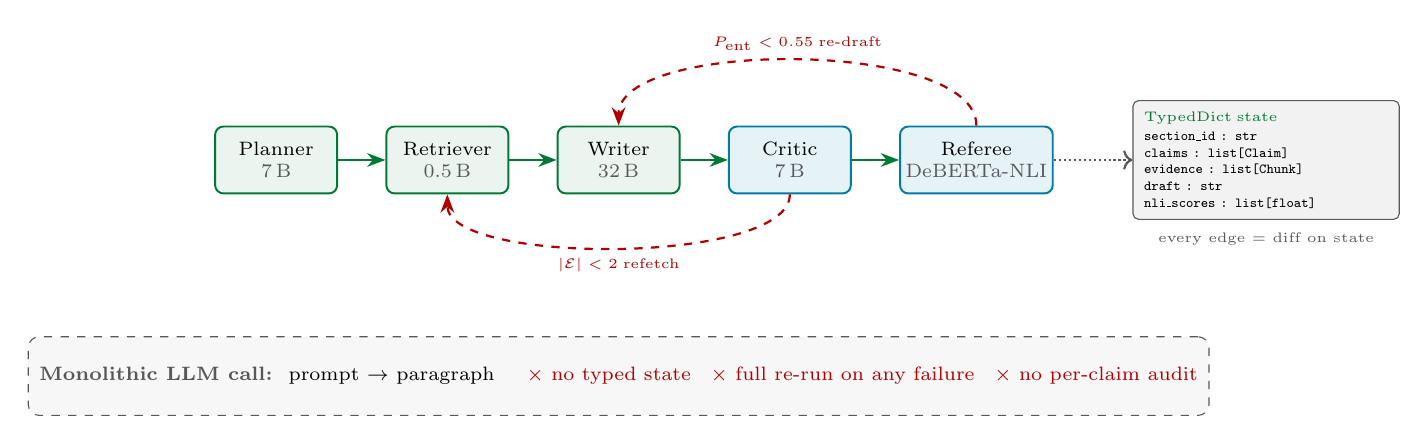
\begin{tikzpicture}[font=\scriptsize,
  node distance=7mm and 6mm,
  agent/.style={draw=ornlgreen,fill=ornlgreen!8,rounded corners=3pt,
                minimum width=1.55cm,minimum height=0.85cm,align=center,
                text=ornlblack,line width=0.7pt,inner sep=2pt},
  gate/.style ={draw=cerulean,fill=cerulean!10,rounded corners=3pt,
                minimum width=1.55cm,minimum height=0.85cm,align=center,
                text=ornlblack,line width=0.7pt,inner sep=2pt},
  state/.style={draw=ornlgrey,fill=ornlgrey!8,rounded corners=2pt,
                font=\tiny\ttfamily,align=left,inner sep=4pt,text=ornlblack},
  flow/.style ={-Stealth,ornlgreen,thick},
  rej/.style  ={-Stealth,red!70!black,thick,dashed},
  cb/.style   ={draw=backgroundgrey,thin,rounded corners=2pt,
                fill=white,inner sep=3pt,font=\tiny,text=ornlgrey,align=center},
  mono/.style ={draw=ornlgrey,dashed,fill=ornlgrey!5,rounded corners=4pt,
                minimum width=11.5cm,minimum height=1.0cm,align=center,
                text=ornlblack,inner sep=4pt}]

  %% ── Row of 5 typed agents (centred at y=0) ─────────────────────
  \node[agent] (P) at (0,0)             {Planner\\\scriptsize\color{ornlgrey}7\,B};
  \node[agent,right=of P] (R)           {Retriever\\\scriptsize\color{ornlgrey}0.5\,B};
  \node[agent,right=of R] (W)           {Writer\\\scriptsize\color{ornlgrey}32\,B};
  \node[gate, right=of W] (C)           {Critic\\\scriptsize\color{ornlgrey}7\,B};
  \node[gate, right=of C] (F)           {Referee\\\scriptsize\color{ornlgrey}DeBERTa-NLI};

  %% forward flow
  \draw[flow] (P)--(R); \draw[flow] (R)--(W);
  \draw[flow] (W)--(C); \draw[flow] (C)--(F);

  %% conditional re-draft / refetch loops (above the row)
  \draw[rej] (F.north) .. controls +(0,1.1) and +(0,1.1) ..
             node[above,font=\tiny,text=red!70!black]
             {$P_{\mathrm{ent}}<0.55$\;re-draft}
             (W.north);
  \draw[rej] (C.south) .. controls +(0,-0.9) and +(0,-0.9) ..
             node[below,font=\tiny,text=red!70!black]
             {$|\mathcal{E}|<2$\;refetch}
             (R.south);

  %% ── TypedDict shared state (to the right of the row) ───────────
  \node[state,right=10mm of F,text width=3.1cm,yshift=0mm]
    (S){\textbf{\color{ornlgreen}\normalfont TypedDict state}\\[1pt]
        section\_id : str\\
        claims      : list[Claim]\\
        evidence    : list[Chunk]\\
        draft       : str\\
        nli\_scores : list[float]};
  \draw[->,ornlgrey,thick,densely dotted] (F.east) -- (S.west);
  \node[font=\tiny,text=ornlgrey,below=1pt of S]{every edge = diff on state};

  %% ── Left callout: localized failure ────────────────────────────
  % \node[cb,left=6mm of P,text width=1.7cm]
    % {\bfseries fault isolated\\\normalfont to one node};

  %% ── Bottom contrast: monolithic LLM ────────────────────────────
  \node[mono,below=18mm of W] (M)
    {\textbf{\color{ornlgrey}Monolithic LLM call:}\;
     prompt $\rightarrow$ paragraph\;\;\;\;
     \color{red!70!black}$\times$ no typed state\;\;
     \color{red!70!black}$\times$ full re-run on any failure\;\;
     \color{red!70!black}$\times$ no per-claim audit};
\end{tikzpicture}}
\end{frame}



\note{We may be wondering why build this as a graph rather than a Chain of Though call? Because a graph gives us fine-grained control over the workflow. Each step can be executed independently, and conditional loops allow revisions flows.  The workflow auditable, enabling every claim to be traced back to its supporting evidence. 

% Everysentence is on auditable graph execution
}




%% ═══════════════════════════════════════════════════════════════
%% 7b — VALIDATION: LINE-BY-LINE vs HUMAN EXPERT PAPER
%% ═══════════════════════════════════════════════════════════════
\begin{frame}{Backup: Validation Protocol: Every Sentence Is Scored Against a Human Expert}
\begin{columns}[T]
  \begin{column}{0.49\textwidth}
    \textbf{\color{ornlgreen}Alignment protocol}\\[2pt]
    {\footnotesize
    \textbf{1.} Split human \& pipeline drafts into sentences.\\
    \textbf{2.} For each $p_j$ find nearest $h_{\pi(j)}$ in MPNet space.\\
    \textbf{3.} Score the pair on three axes:
    }\\[4pt]
    {\footnotesize
    \;$\bullet$ \textbf{Entailment} $E_j$ — DeBERTa-v3 NLI\\
    \;$\bullet$ \textbf{Numeric error} $N_j{=}|\hat y_j{-}y_j|/|y_j|$\\
    \;$\bullet$ \textbf{Citation overlap} $C_j$
    }\\[4pt]
    {\footnotesize Accept iff $E_j{\geq}0.55 \wedge N_j{\leq}0.10
     \wedge C_j{\geq}0.5$.}
  \end{column}
  \begin{column}{0.49\textwidth}
    \textbf{\color{backgroundgreen}What each metric means}\\[2pt]
    {\footnotesize
    \;$\bullet$ \textbf{Recall} $=$ \% of human claims we found.\\
    \;$\bullet$ \textbf{Precision} $=$ \% of our claims that match human.\\
    \;$\bullet$ \textbf{Faithfulness} $=$ NLI agreement to source chunks.\\
    \;$\bullet$ \textbf{Citation grounding} $=$ \% of cited values
     with a verified bbox.\\
    \;$\bullet$ \textbf{JSD} $=$ topic-distribution divergence
     (0 $=$ identical emphasis).\\
    \;$\bullet$ \textbf{NMAE} $=$ normalized numeric error.}\\[4pt]
    {\scriptsize\color{ornlgrey}
    Ground truth: 30-page expert review on Li$_2$TiO$_3$ breeders.
    614 H \,|\, 587 P \,|\, 478 aligned pairs.}
  \end{column}
\end{columns}
\end{frame}
\note{We verify quality against a 30-page expert review on lithium titanate breeders (614 human sentences vs. 587 generated). Each generated sentence is matched to the closest human sentence in embedding space, then checked on three criteria: NLI entailment (DeBERTa), numeric accuracy, and citation overlap. A sentence is accepted only if it passes all three thresholds.}





\end{document}

